\chapter{Resultados y discusi\'on}
\label{ch:resultadosRadio}

El objetivo de este cap\'itulo (y de la segunda parte de esta tesis) es estimar el desempe\~no  de un detector de antenas de radio a la hora de detectar neutrinos ES.
Para ello, al igual que en Auger se calcular\'a la exposici\'on del detector en un caso gen\'erico.
Se utilizar\'a lo aprendido en el capitulo \ref{ch:caracterizacionRadio} para definir un criterio de disparo y se estimar\'an las eficiencias de detecci\'on.
Todo lo anterior se realizar\'a utilizando distintas disposiciones espaciales de las antenas (topograf\'ias del detector), para encontrar una disposici\'on \'optima.
Finalmente, teniendo en cuenta todo lo anterior se comparar\'a el desempe\~no que puede alcanzar un detector de radio frente a la pr\'oxima generaci\'on de detectores de neutrinos ultra energ\'eticos.

\section{C\'alculo de la exposici\'on}
	
	Para calcular la exposici\'on en el detector se utiliz\'o una modificaci\'on de la ecuaci\'on \ref{eq:exp5ES} de la secci\'on \ref{sc:expoNu}, con la que se obtuvo la exposici\'on a neutrinos ES en Auger.
	Tales modificaciones fueron necesarias debido a que:
	\begin{enumerate}
	 \item Se incluy\'o la curvatura de la tierra en el c\'alculo de la exposici\'on.
	 \item Las eficiencias se calcularon en funci\'on de la energ\'ia visible.
	 \item Se considera un detector ideal, que no var\'ia a trav\'es del tiempo ni en su forma.
	\end{enumerate}
	%
	Estos tres puntos implican cambios en el t\'ermino de probabilidad, en las eficiencias y en las integrales que se deben realizar.
	Por este motivo las siguientes secciones se avocan a desarrollarlos en detalle.
	
% 	\begin{equation}
% 		\begin{aligned}
% 		{\cal E}_{ES}(E_\nu)\equiv2\pi\iiint\limits_{E_v~{\rm x_d}~\theta}P({\rm x_d},E_v|E_{\nu},\theta)~
% 		\left[~
% 		\iint\limits_{T~A}\epsilon({\rm x_d},E_v,A,\theta_D,T)~dA~dT
% 		\right]\\
% 		~\sen\theta_D d\theta_D~d{\rm x_d}~dE_v
% 		\end{aligned}
% 	 \label{eq:exp1ESRadio}
% 	\end{equation}
% 	%

	\subsection{Inclusi\'on de la curvatura de la tierra}
	El primer cambio en el c\'alculo es inducido por la inclusi\'on de la curvatura de la tierra en el modelo. 
	Esto resulta en que el \'angulo cenital con el que los neutrinos atraviezan la tierra, \te{}, difiere del observado sobre el detector \td{}, tal como se esquematiza en la figura \ref{fig:curveEarthSketch0}.
	%
	 \begin{figure}[ht!]
		\centering
		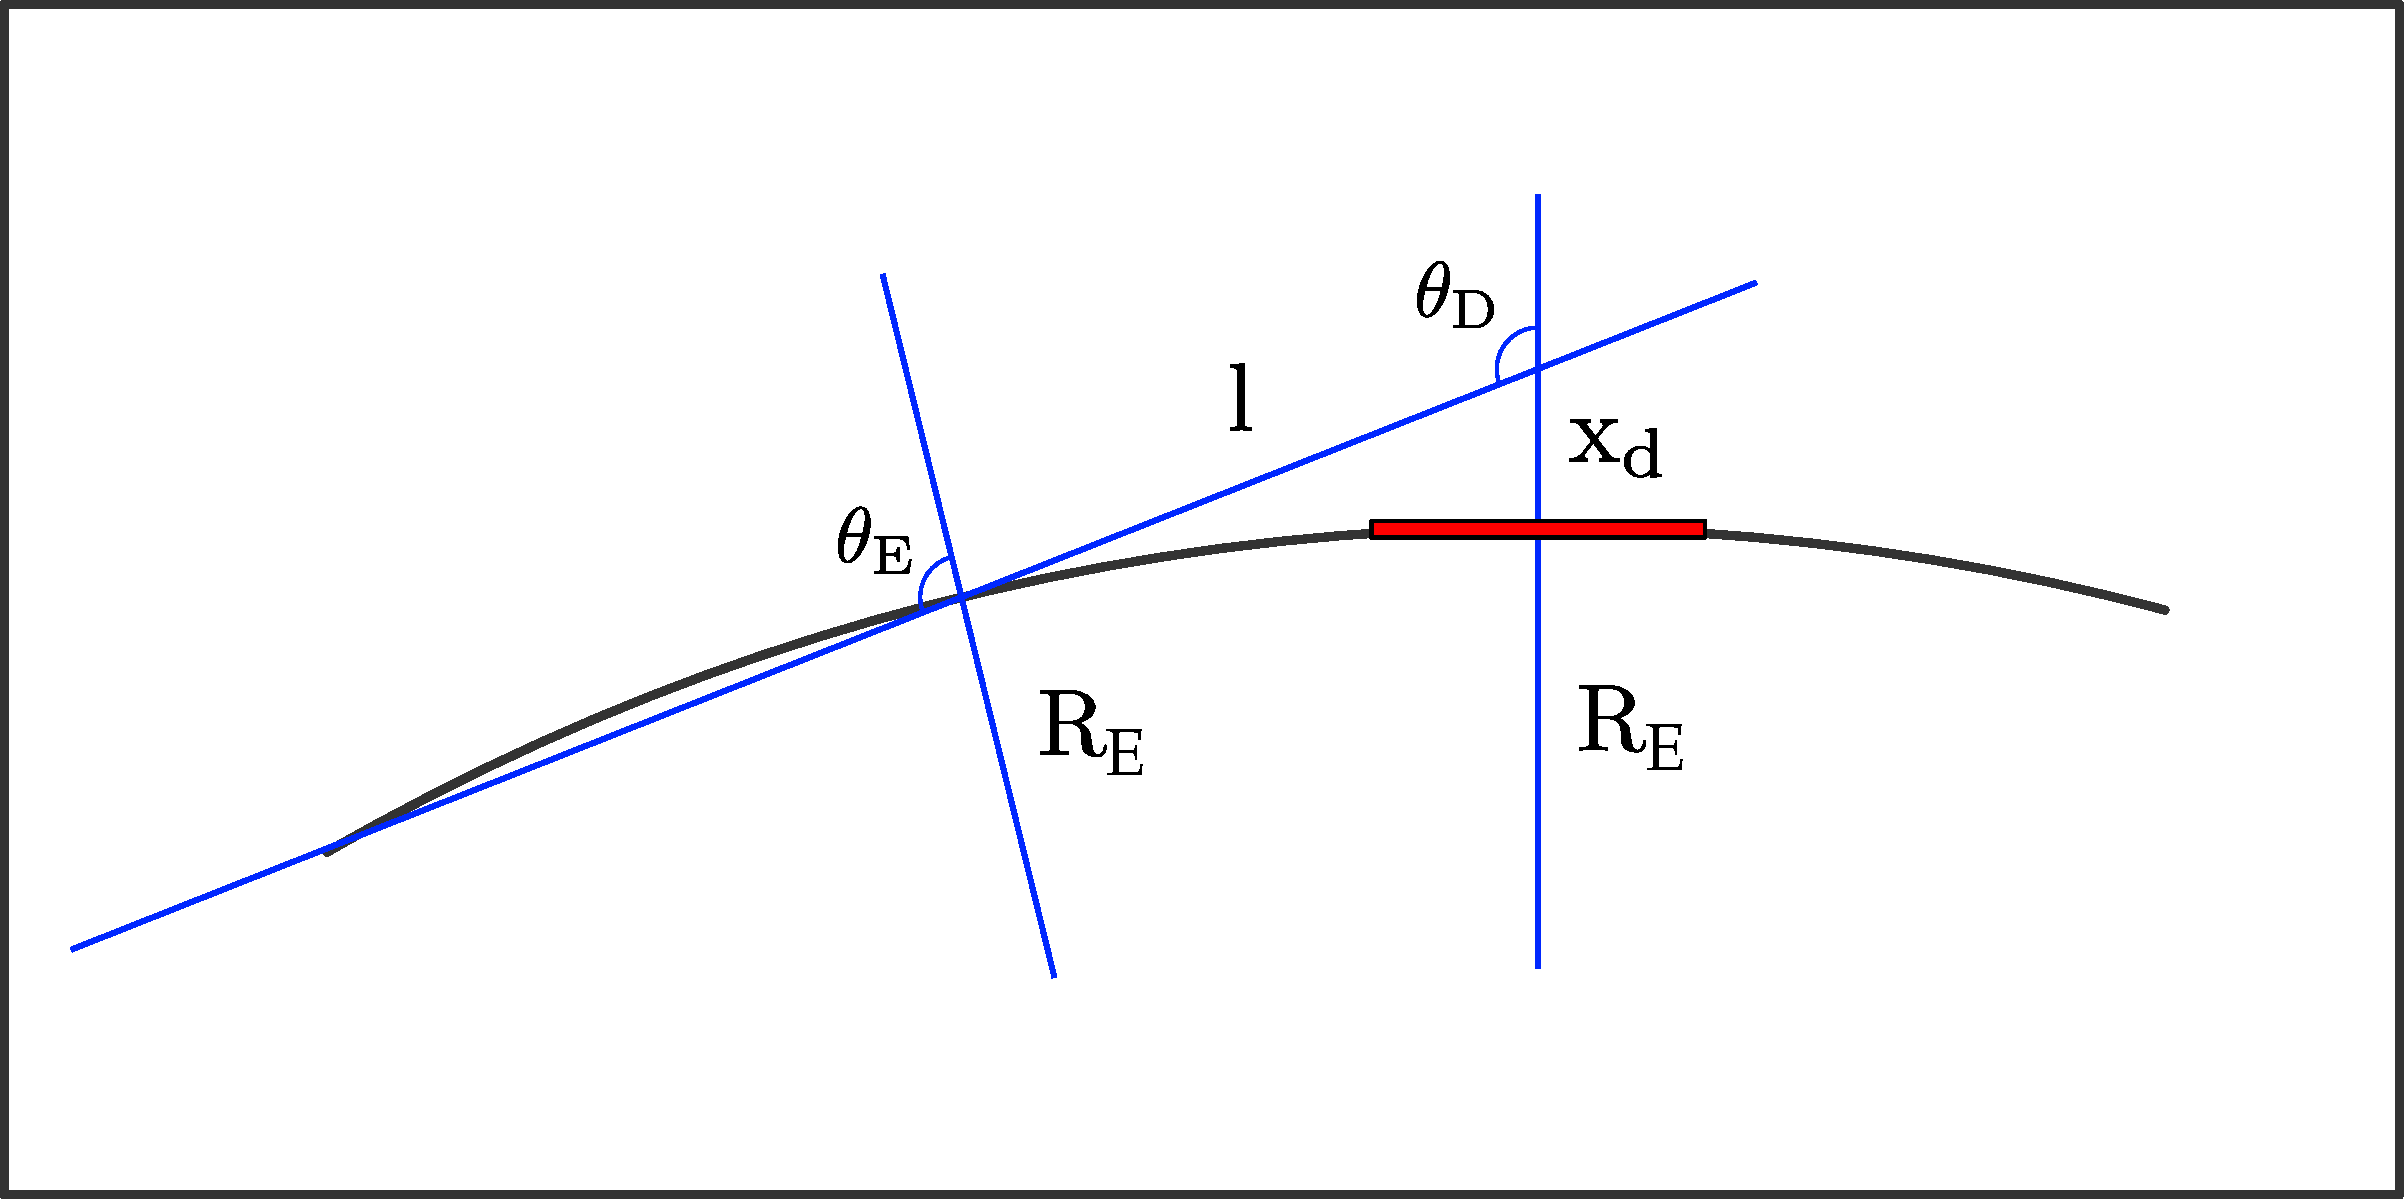
\includegraphics[width=0.8\textwidth]{./fig/appendix/curveEarthSketch.pdf}
		\caption{\label{fig:curveEarthSketch0}
		Esquema del cambio en el angulo sobre el detector y el utilizado para calcular las probabilidades de interacci\'on del neutrino en la tierra.
		}
	\end{figure}
	%
	Como consecuencia el c\'alculo se ve afectdo de dos maneras:
	\begin{enumerate}
	 \item Se modifican las probabilidades de decaimiento del \tauon{} en la atm\'osfera.
	 \item Para cada valor de \xd{} existe una zona de \'angulos cenitales prohibidos.
	\end{enumerate}
	
	\subsubsection{Cambio en las probabilidades de decaimiento en la atm\'osfera}
	Tal como se discuti\'o en la secci\'on \ref{sbsc:corrES}, el decaimiento del \tauon{} en la atm\'osfera se puede modelar como una distribuci\'on exponencial, de forma:
	%
	\begin{equation}
		h({\rm x_d},(E_\tau,\theta_D))=
		\exp{\left(
		-\frac{l({\rm x_d},\theta_D)}{\lambda(E_\tau)}
		\right)}
		\frac{dl({\rm x_d})}{d{\rm x_d}}
		\frac{1}{\lambda(E_\tau)}
		\label{eq:decayTayRadio}
	\end{equation}
	%
	Entonces, si se tiene en cuenta la curvatura de la tierra, la expresi\'on de $l({\rm x_d},\theta_D)$ queda:
	%
	\begin{equation}
		\begin{array}{rcl}
		l({\rm x_d},\theta_D) & = & \dfrac{R_E^2-(R_E+{\rm x_d})^2}{R_E \cos \theta_E + (R_E+{\rm x_d}) \cos \theta_D}\\
		&&\\
		\end{array}
		\label{eq:l_curve0}
	\end{equation}
	donde $R_E$ es el radio de la tierra y:
	\begin{equation}
		\begin{array}{rcl}
		\cos \theta_E & = & - \left[ \dfrac{R_E^2 - (R_E+{\rm x_d})^2 (1-\cos^2 \theta_D)}{R_E^2} \right]^{\frac{1}{2}} \\ 
		\end{array}
		\label{eq:te_td0}
	\end{equation}
	%
	Luego, derivando \ref{eq:l_curve0} puede obtenerse anal\'iticamente la expresi\'on de $\frac{dl({\rm x_d})}{d{\rm x_d}}$:
	\begin{equation}
	\begin{aligned}
		\frac{dl({\rm x_d})}{d{\rm x_d}}
		=&-
		\frac{
		2(R_E+{\rm x_d})
		(R_E\cos{\theta_E}+(R_E+{\rm x_d}\cos{\theta_D}))
		}{
		(R_E\cos{\theta_E}+(R_E+{\rm x_d}\cos{\theta_D}))^2
		}\\
% 		\ & \\
		&-
		\frac{(R_E^2+(R_E+{\rm x_d})^2)(R_E\frac{d\cos{\theta_E}}{d{\rm x_d}}+\cos{\theta_D})
		}{
		(R_E\cos{\theta_E}+(R_E+{\rm x_d}\cos{\theta_D}))^2
		}
	\end{aligned}
	\end{equation}
	%
	con:
	\begin{equation}
	\frac{d\cos{\theta_E}}{d{\rm x_d}}
	=
	\frac{
	(R_E+{\rm x_d})
	(1-\cos^2\theta_D)
	}{\cos{\theta_E}R_E^2
	}
	\end{equation}
	%
	La derivaci\'on de estas ecuaciones puede encontrarse en el ap\'endice \ref{ap:tierraCurva} junto con un peque\~no an\'alisis de su impacto.
	
	\subsubsection{\'Angulos cenitales prohibidos}
	Por simple geometr\'ia, para cada valor de \xd{} aparecer\'a un \'angulo observado m\'inimo sobre el detector, $\theta_D^{cut}$, correspondiente al m\'inimo valor con el que los neutrinos pueden incidir sobre la tierra, $\theta_E=90^\circ$.
	Esta situaci\'on se bosqueja en la figura \ref{fig:curveEarthSketch_thCut0}.
	%
	\begin{figure}[ht!]
		\centering
		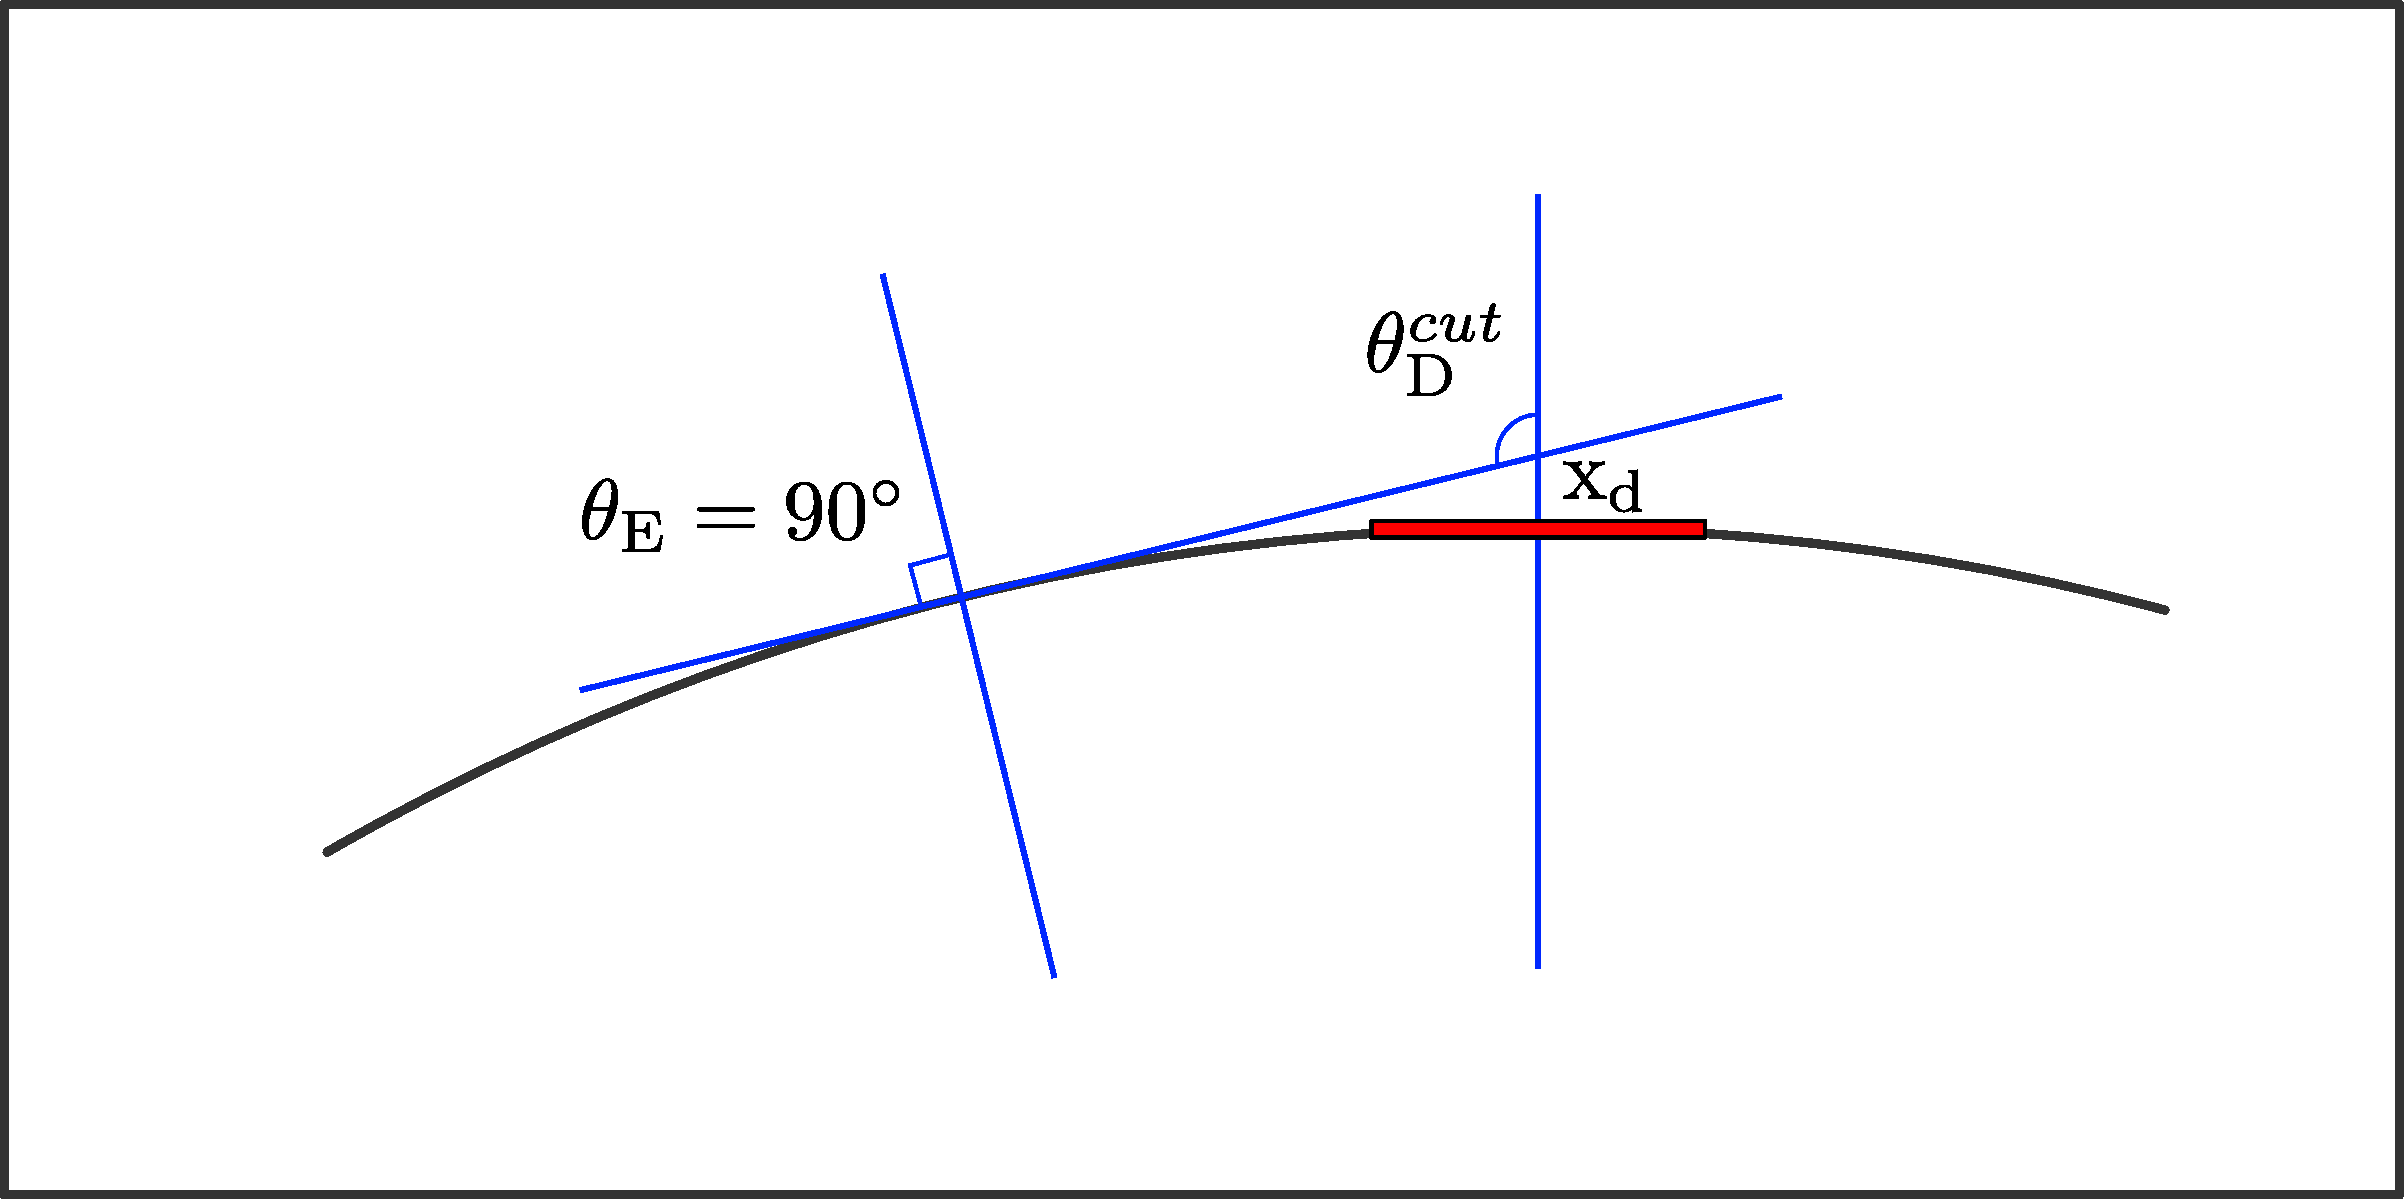
\includegraphics[width=0.8\textwidth]{./fig/appendix/curveEarthSketch_thCut.pdf}
		% curveEarthSketch.png: 2404x1199 pixel, 150dpi, 40.70x20.30 cm, bb=0 0 1154 575
		\caption{\label{fig:curveEarthSketch_thCut0}
		Dado \xd{} existe un valor m\'inimo de \td{}, $\theta_D^{cut}$, que corresponde a $\theta_E=90^\circ$.
		}
	\end{figure}
	%
	Este valor l\'imite puede calcularse anal\'iticamente (ver ap\'endice \ref{ap:tierraCurva}), y su expresi\'on es:
	\begin{equation}
	\cos \theta_D^{cut} = \left[ \frac{2 R_E {\rm x_d}+{\rm x_d}^2}{(R_E+{\rm x_d})^2} \right]^{\frac{1}{2}}
	\label{eq:tdc0}
	\end{equation}
	%
	Entonces, para cada \xd{} pueden calcularse los valores permitidos para \td{}, que se grafican en la figura \ref{fig:dx_thcut0}.
	\begin{figure}[ht!]
		\centering
		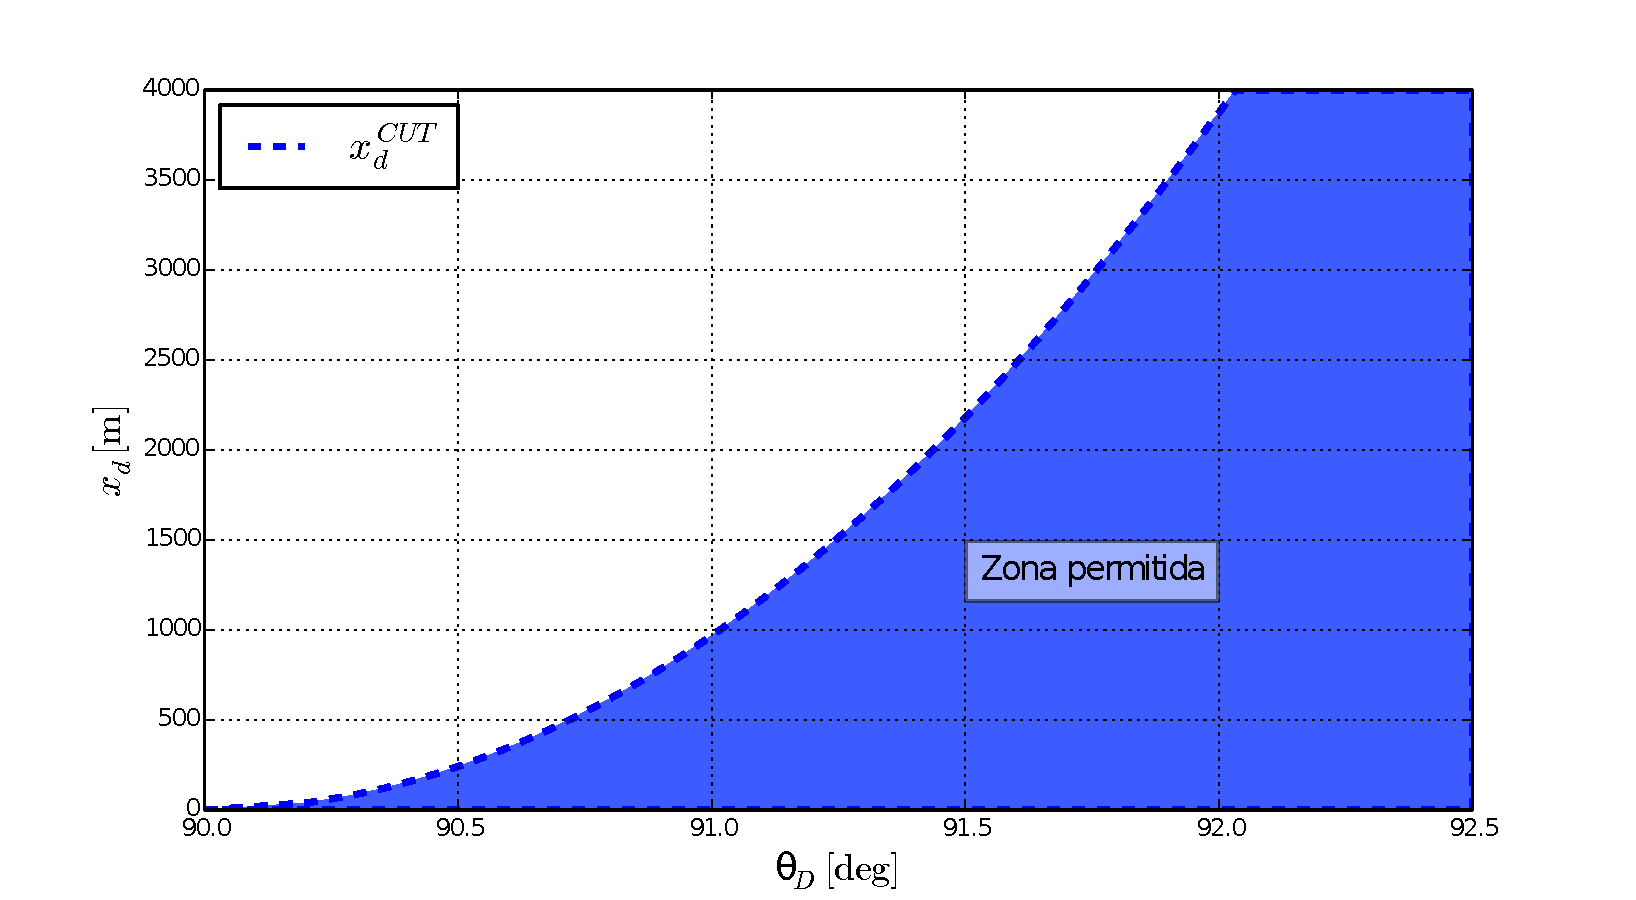
\includegraphics[width=0.95\textwidth]{./fig/appendix/thetaDCut_mod}
		% curveEarthSketch.png: 2404x1199 pixel, 150dpi, 40.70x20.30 cm, bb=0 0 1154 575
		\caption{\label{fig:dx_thcut0}
		Conjunto de par\'ametros geom\'etricamente admitidos.
		}
	\end{figure}
	%
	Si bien este efecto no tiene mucha relevancia en la exposici\'on de Auger\footnote{Esto se debe a que el rango angular en el que Auger es eficiente es de alrededor de $5^\circ$. Entonces, los eventos cuyo \'angulo se ve modificado siguen siendo detectados (ver figura \ref{fig:te_td} del apendice \ref{ap:tierraCurva}).}, tiene un impacto considerable en detectores de radio, cuyo rango angular es cercano a los $2.5^\circ$.
	
	\subsection{Manejo de la energ\'ia visible}
	Las eficiencias de detecci\'on ser\'an calculadas en funci\'on de la energ\'ia visible de la lluvia, \ev{}, por lo que es necesario modificar el c\'alculo de la exposici\'on.
	Recordando las ecuaci\'ones \ref{eq:exp5ES} y \ref{eq:exp5.2ES} del cap\'itulo \ref{ch:resAuger}, en este caso el t\'ermino de probabilidad puede ser escrito de la siguiente manera:
	%
	\begin{equation}
		\begin{aligned}
		P({\rm x_d},E_v|E_{\nu},\theta_D)=
		\int\limits_{E_v}^{E_\nu}
		g(E_v|E_\tau)
		& f(E_\tau|E_\nu,\theta_E(\theta_D,{\rm x_d}))\\
		&h({\rm x_d},(E_\tau,\theta_D))
		|\cos\theta_D|
		dE_\tau
		\end{aligned}
	\end{equation}
	%
	donde la funci\'on $f(E_\tau|E_\nu,\theta_E(\theta_D,{\rm x_d}))$ nuevamente describe la probabilidad de obtener un \tauon{} emergente de energ\'ia \etau{}, dado que incidi\'o un neutrino sobre la tierra de par\'ametros $E_\nu,\theta_E(\theta_D,{\rm x_d})$ y al igual que en Auger se calcularon mediante simulaciones de Monte Carlo.
	Por otro lado, $h({\rm x_d},(E_\tau,\theta_D))$ es la de la ecuaci\'on \ref{eq:decayTayRadio} y $g(E_v|E_\tau)$ representa la probabilidad de que un evento tenga energ\'ia \ev{} dado que fue iniciado por el dacimiento de un \tauon{} de energ\'ia \etau{}.
	En lugar de $g(E_v|E_\tau)$, para realizar la integral se calcul\'o $\tilde{g}(\log E_v-\log E_\tau)$ a partir de la librer\'ia de \tauola{} utilizada para simular los decaimientos del \tauon{} en Auger.
	Esta funci\'on se muestra entre $-3$ y $0$ en la figura \ref{fig:ev_etau} en la que se observa que aproximadamente el $95\%$ de los casos obtienen una energ\'ia visible en el mismo orden de magnitud que la del \tauon{}.
	%
	 \begin{figure}[h!]
		\begin{center}
			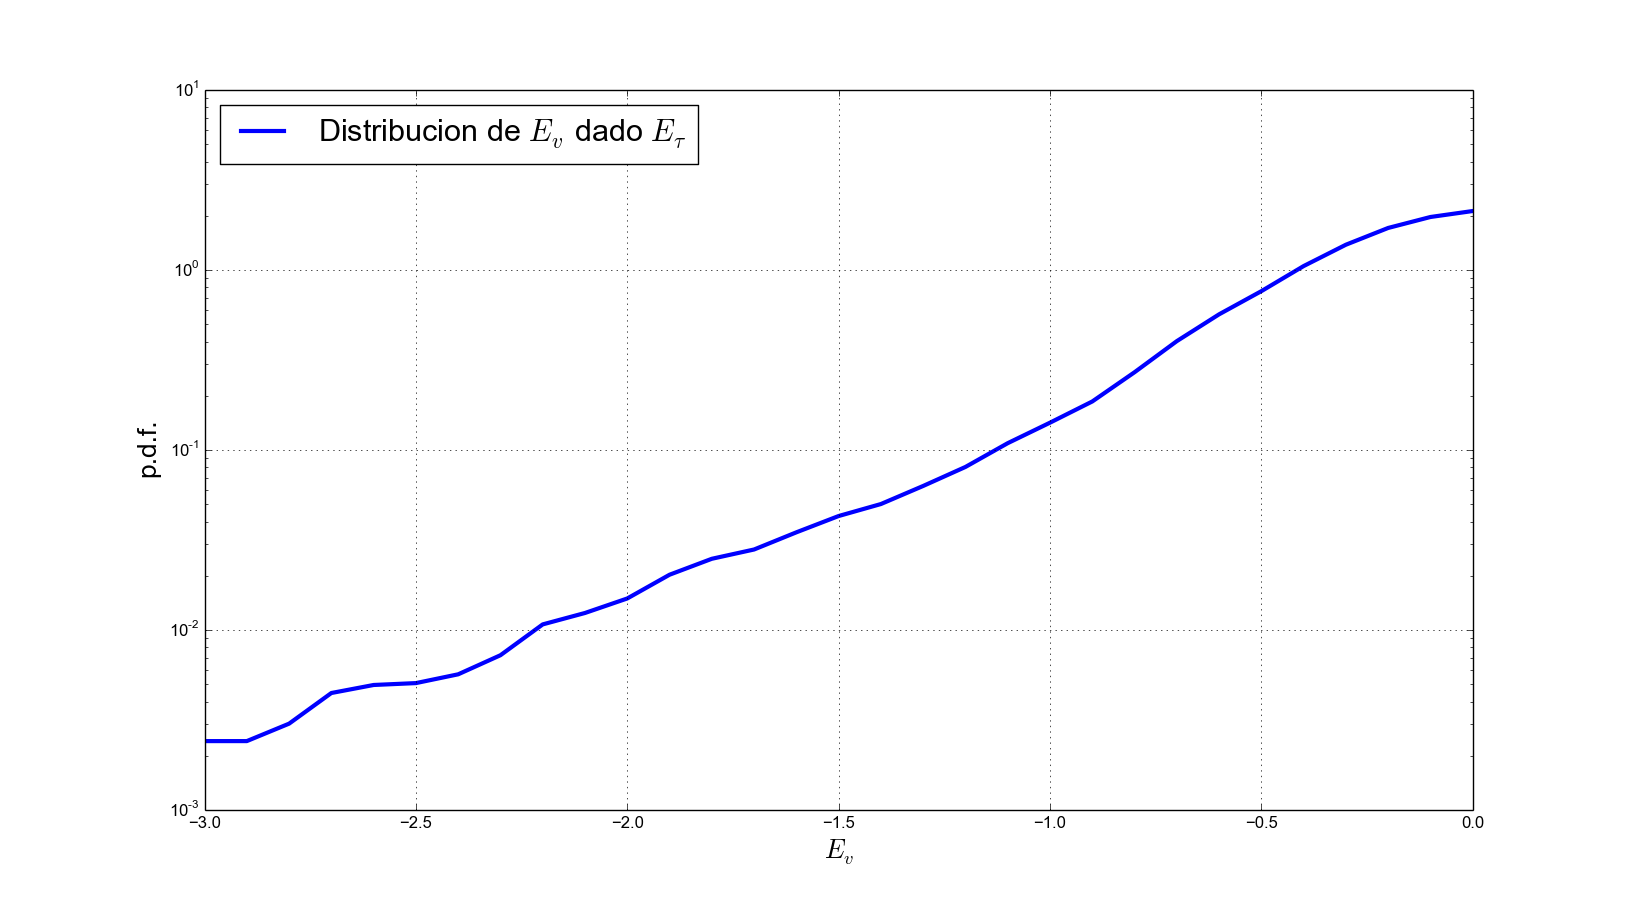
\includegraphics[width=0.9\textwidth]{fig/resultadosRadio/ev_etau}
			\caption{\label{fig:ev_etau} 
			Distribuci\'on de \ev{} dado \etau{} obtenida a partir de los decaimientos simulados con \tauola{}. 
			}
		\end{center}
	\end{figure}
	 
	\subsection{Integraci\'on temporal y espacial}
	Finalmente, dado que esta parte de la tesis se enfoca en un detector gen\'erico, no ser\'a necesario realizar la integral por unidad de tiempo y \'area y simplemente se multiplicar\'a por un factor \cant{T\ A=1}{s cm^2} o en caso de que se pretenda comparar con un detector, se utilizar\'a el factor correspondiente.
	
	Teniendo en cuenta todo lo anterior, la ecuaci\'on para calcular la exposici\'on resulta:
	%
	\begin{equation}
		\begin{aligned}
			{\cal E} (E_\nu) = 2 \pi T A
			\int_{0}^{\infty} 
			\int_{\theta_D^{cut}}^{\theta_D^{max}} 
			\int_{0}^{E_\nu} 
			\int_{0}^{E_\tau} 
			\epsilon ({\rm x_d},\theta_D,E_v)& 
			\frac{e^{\frac{l({\rm x_d})}{\lambda(E_\tau)}}}{\lambda(E_\tau)}\frac{dl({\rm x_d})}{d{\rm x_d}}
			\tilde{g}(\log E_v-\log E_\tau)\\
			f(E_\tau|E_\nu,\theta_E(\theta_D,{\rm x_d}))
			&\sin \theta_D |\cos \theta_D|
			dE_v dE_\tau  d\theta_D d{\rm x_d}
		\end{aligned}
		\label{eq:exp2ESRadio}
	\end{equation}

	Una vez obtenidas las eficiencias (ver secci\'on \ref{sc:effRadio}) esta integral se computa numericamente.
	
	
\section{Detector ideal - Rendimiento de la corteza terrestre como blanco}
	Antes de pasar al c\'alculo de las eficiencias de detecci\'on, es interesante estudiar las capacidades que tendria un detector ideal, es decir, que detecte todos los eventos iniciados por neutrinos ES que emerjan de la tierra.
	Para ello, se calcul\'o la integral de la ecuaci\'on \ref{eq:exp2ESRadio} bajo la condici\'on $\epsilon ({\rm x_d},\theta_D,E_v) = 1$ y $TA=1$, para diferentes valores de $\theta_D^{max}$.
% 	Recordando la ecuaci\'on \ref{eq:exp0} del cap\'itulo \ref{ch:resAuger}, 
	En la figura \ref{fig:exposuresFluxThetas} se grafica esta cantidad multiplicada por $E_\nu^{-2}$, lo que, recordando la ecuaci\'on \ref{eq:exp0} del cap\'itulo \ref{ch:resAuger}, se debe integrar en $E_\nu$ para obtener la cantidad de eventos por unidad de \'area y tiempo bajo la condici\'on de \cant{k=1}{GeV\ s^{-1}\ sr^{-1}\ cm^{-2}}.
%
	\begin{figure}[h!]
		\begin{center}
			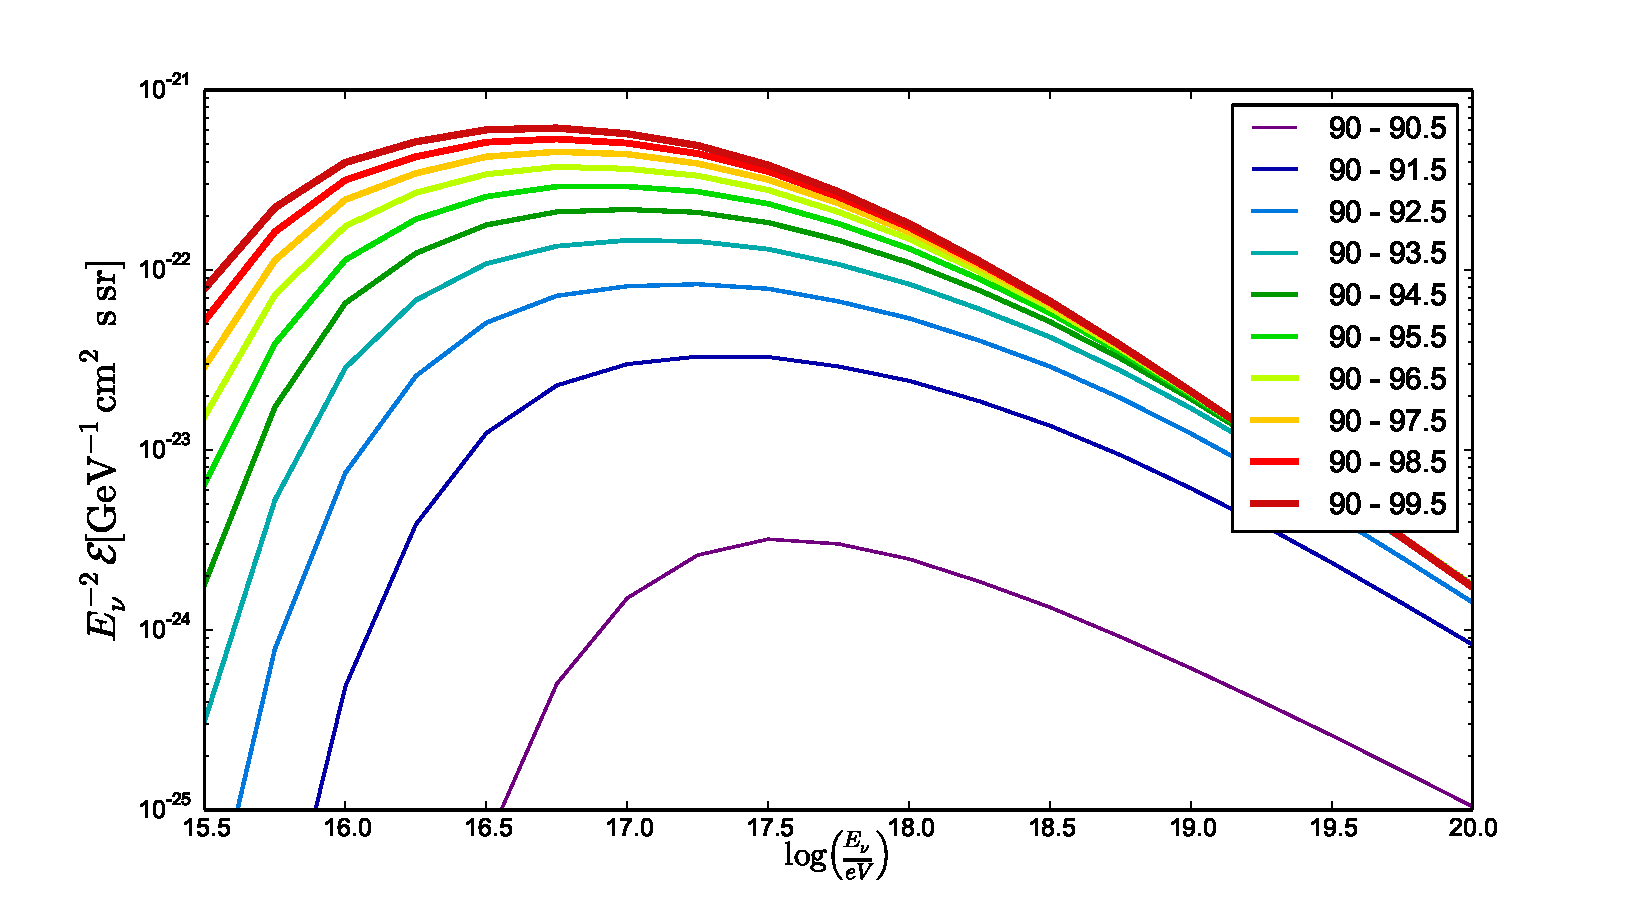
\includegraphics[width=0.9\textwidth]{fig/resultadosRadio/exposureFullEff_thetas}
			\caption{\label{fig:exposuresFluxThetas} Eventos esperados sobre el detector por unidad de \'area y tiempo para un flujo $\phi(E_\nu)= E^{-2}{\rm GeV\ s^{-1}\ sr^{-1}\ cm^{-2}}$, en funci\'on de la energ\'ia y suponiendo eficiencia m\'axima en el rango angular indicado.
			Naturalmente, la cantidad esperados aumenta a medida que lo hace el rango angular del \emph{detector ideal}.
			}
		\end{center}
	\end{figure}
	%
	Como era de suponerse, a medida que aumenta el rango angular de detecci\'on la cantidad de eventos esperados por unidad de energ\'ia aumenta.
	Por otro lado, dado el rango angular, estas curvas representan la sensibilidad en energ\'ia del blanco.
	Puede notarse como a medida que aumenta $\theta_D^{max}$ el m\'aximo de la curva se desplaza hacia energ\'ias m\'as bajas.
	Este fen\'omeno se debe a que mientras mayor es el \'angulo de incidencia, los neutrinos m\'as energ\'eticos interactuar\'an en promedio m\'as lejos del lugar de escape hacia la atm\'osfera que los menos energ\'eticos, lo que le quita probabilidad de escapar al \tauon{} resultante.
	
	Ademas de la forma, para comparar la normalizaci\'on de las curvas, que es proporcional a la cantidad de eventos esperados, se puede realizar la integral en $E_\nu$ de cada una, lo que se muestra en la figura \ref{fig:gainThetas} en unidades de la integral obtenida para el rango angular del detector de radio ($N_{92.5}$). 
	%
	\begin{figure}[h!]
		\begin{center}
			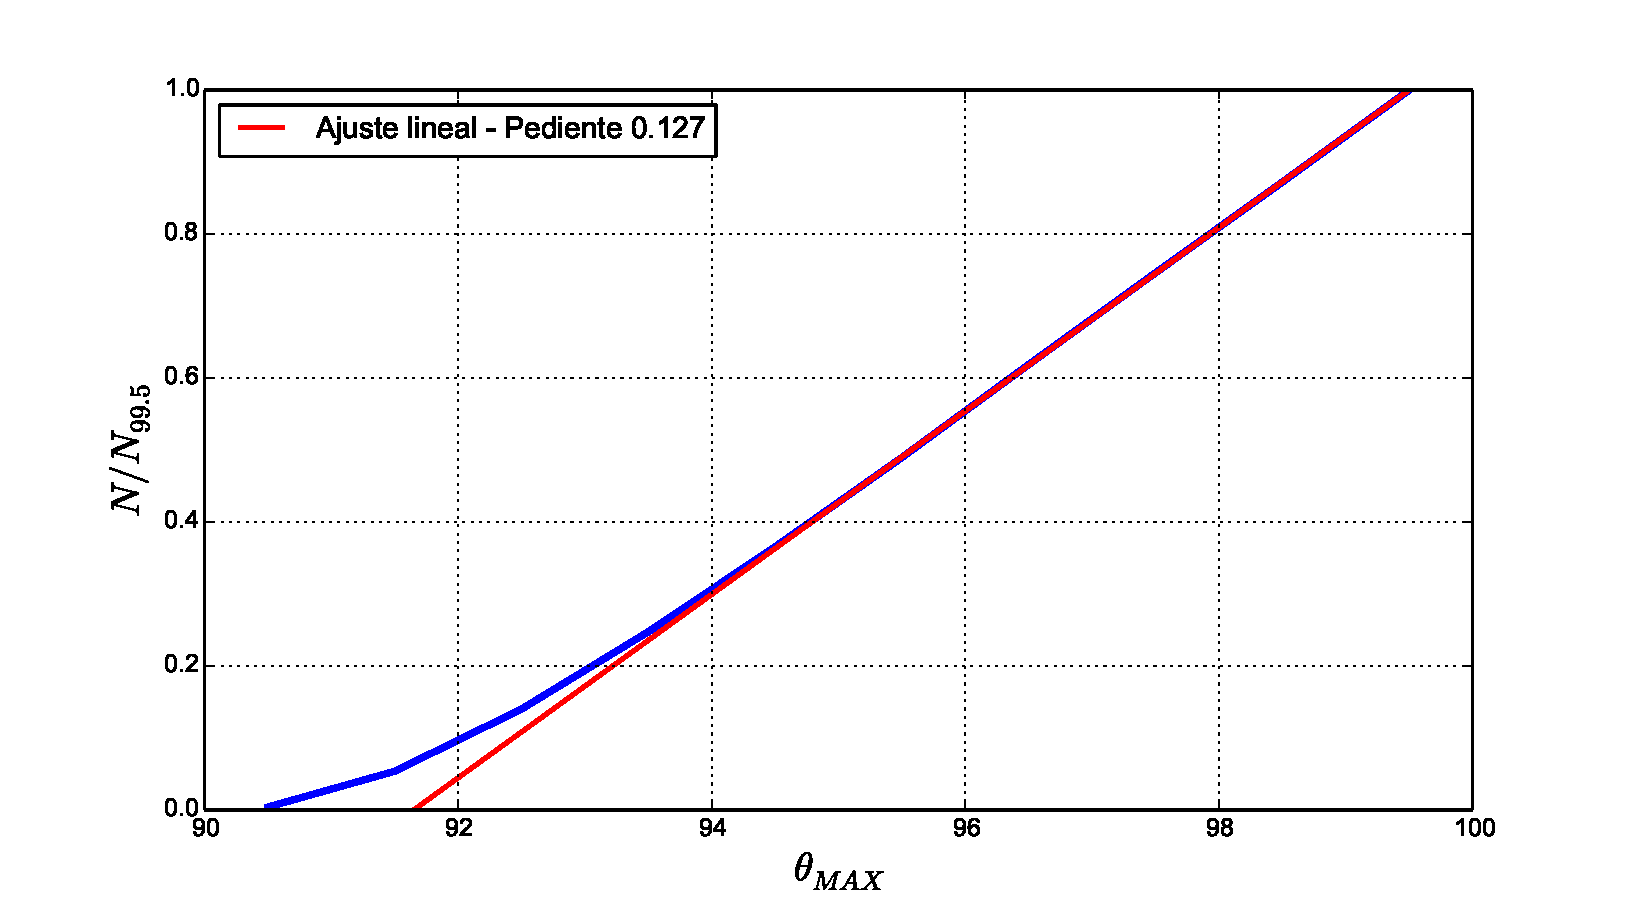
\includegraphics[width=0.9\textwidth]{fig/resultadosRadio/eventGain_thetas}
			\caption{\label{fig:gainThetas} Cantidad de eventos esperados como funci\'on del m\'aximo del rango angular, en relaci\'on al calculado para el del detector de radio ($N_{92.5}$).
			En rojo se grafica un ajuste lineal de pendiente 0.908, que aproxima la curva para valores de $\theta_{MAX}>94$.
			Esto quiere decir que cada grado por encima de $94^\circ$ aporta una cantidad constante eventos sobre el detector.
			}
		\end{center}
	\end{figure}
	%
	La primer observaci\'on interesante sobre la figura es que la relaci\'on entre $N(95^\circ)$ y $N(92.5^\circ)$ es aproximadamente 3.
	Esto quiere decir que en principio el detector de superficie de Auger tiene la capacidad de detectar el triple de eventos que uno equivalente basado en la t\'ecnica de radio.
	Esta desventaja debe ser compensada por un aumento significativo en el \'area instrumentada.
	
	Adem\'as, en la figura se muestra una recta de pendiente 0.908 obtenida mediante un ajuste lineal para los valores de $\theta_{MAX}>94$.
	Esto quiere decir que cada grado por encima de $94^\circ$ aporta una cantidad constante eventos sobre el detector (un $90\%$ de lo esperado para $\theta_{MAX}=92.5^\circ$).
	
\section{Obtenci\'on de las eficiencias}
\label{sc:effRadio}

Para calcular la integral de la ecuaci\'on \ref{eq:exp2ESRadio} son necesarias las eficiencias de detecci\'on a neutrinos en funci\'on de los par\'ametros $E_v$, $\theta_D$ y ${\rm x_d})$. Para ello fueron necesarios los siguientes pasos:
%
	\begin{enumerate}
	 \item Especificar el espacio de par\'ametros en el que las eficiencias ser\'ian calculadas para definir qu\'e eventos hacia falta simular.
	 \item Definir el criterio de disparo global y aplicarlo a diferentes topograf\'ias del detector.
	 \item Estimar las eficiencias de identificaci\'on.
	\end{enumerate}

	
	\subsubsection{Pesos de las lluvias}
	Para determinar qu\'e bines (conjunto de valores $E_v$, $\theta_D$ y ${\rm x_d}$) se deben simular se calcul\'o el peso relativo que tendr\'ia cada uno en la integral \ref{eq:exp2ESRadio} dado un flujo $\Phi(E_\nu)\propto E_\nu^{-2}$.
	Esto es equivalente a calcular la probabilidad relativa de ocurrencia de eventos en funci\'on de los par\'ametros $(E_v,\theta_D,{\rm x_d})$, lo que viene dado por la integral de la ecuaci\'on \ref{eq:weightsRadio}.
	%
	\begin{equation}
		\begin{aligned}
			P_\nu(E_v,\theta_D,{\rm x_d})
			\propto
			\sin{\theta_D}|\cos{\theta_D}|
			\iint_{E_\tau,E_\nu}&
			\frac{e^{\frac{l({\rm x_d})}{\lambda(E_\tau)}}}{\lambda(E_\tau)}\frac{dl({\rm x_d})}{d{\rm x_d}}
			%P({\rm x_d}|E_\tau;\theta_D)
			\tilde{g}(\log E_v-\log E_\tau)\\
			%P(\log{E_v}|\log{E_\tau})\\
			&f(E_\tau|E_\nu,\theta_E(\theta_D,{\rm x_d}))
			%&P(\log{E_\tau}|\log{E_\nu})
			E_\nu^{-2}
			dE_\tau dE_\nu
		\end{aligned}
		\label{eq:weightsRadio}
	\end{equation}
	%
	Recordando el significado probabil\'istico de cada uno de los factores, resulta evidente que el valor de dicha integral, para cierto conjunto de par\'ametros $(E_v^*,\theta_D^*,{\rm x_d}^*)$, es proporcional a la cantidad de eventos que se espera en las cercanias de ese punto del espacio de fases\footnote{Las integrales en $E_\nu$ y $E\tau$ dan cuenta de la suma sobre todos los neutrinos y taus que dan lugar a eventos de par\'ametros $(E_v^*,\theta_D^*,{\rm x_d}^*)$.}.
	As\'i, con esta medida es posible establecer la importancia relativa entre diferentes bines.
	
	La figura \ref{fig:radioShWeights} muestra el resultado de esta integral para diferentes varios valores de $E_v$, $\theta_D$ y ${\rm x_d})$.
	Se observa un decaimiento a medida que aumenta \xd{}, lo que es compatible con la probabilidad exponencial en la atm\'osfera. 
	Sin embargo a medida que aumenta la energ\'ia este se atenua, lo que es compatible con el hecho de que la longitud de decaimiento es proporcional a la energ\'ia del \tauon{}.
	Por otro lado, comprender el comportamiento en funci\'on de \td{} y \ev{} resulta complicado ya que mezcla la dependencia de las pdf (funcion $f(E_\tau|E_\nu,\theta_E(\theta_D,{\rm x_d}))$), el efecto de la tierra curva y el flujo de neutrninos, supuesto $\propto E^{-2}$.
	No obstante, este ultimo factor parece ser relevante ya que entre \cant{10^{16.25}}{eV} y \cant{10^{18.25}}{eV} los pesos caen en tres \'ordenes de magnitud.
	Por este motivo no se podndran esfuerzos en calcular con detalle las eficiencias por encima de \cant{10^{18}}{eV} y se las aproximar\'a por las obtenidas para este valor.
	%
	\begin{figure}[ht!]
		\centering
		\begin{tabular}{cc}
		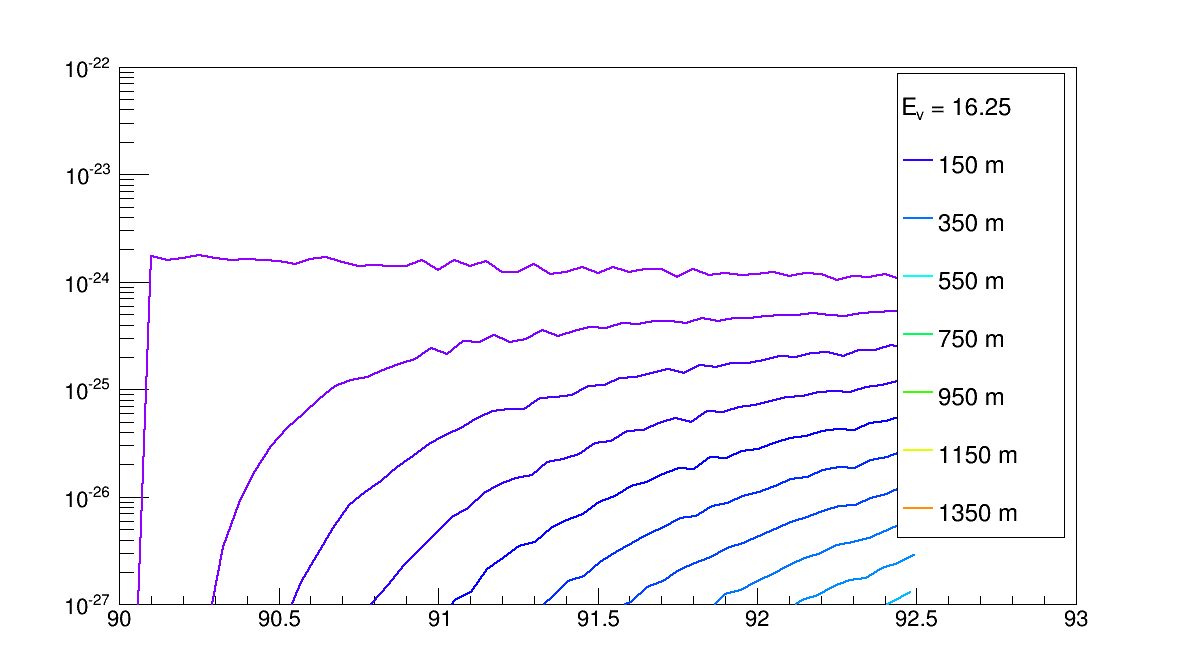
\includegraphics[width=0.45\textwidth]{fig/resultadosRadio/weights16_25.png} &
		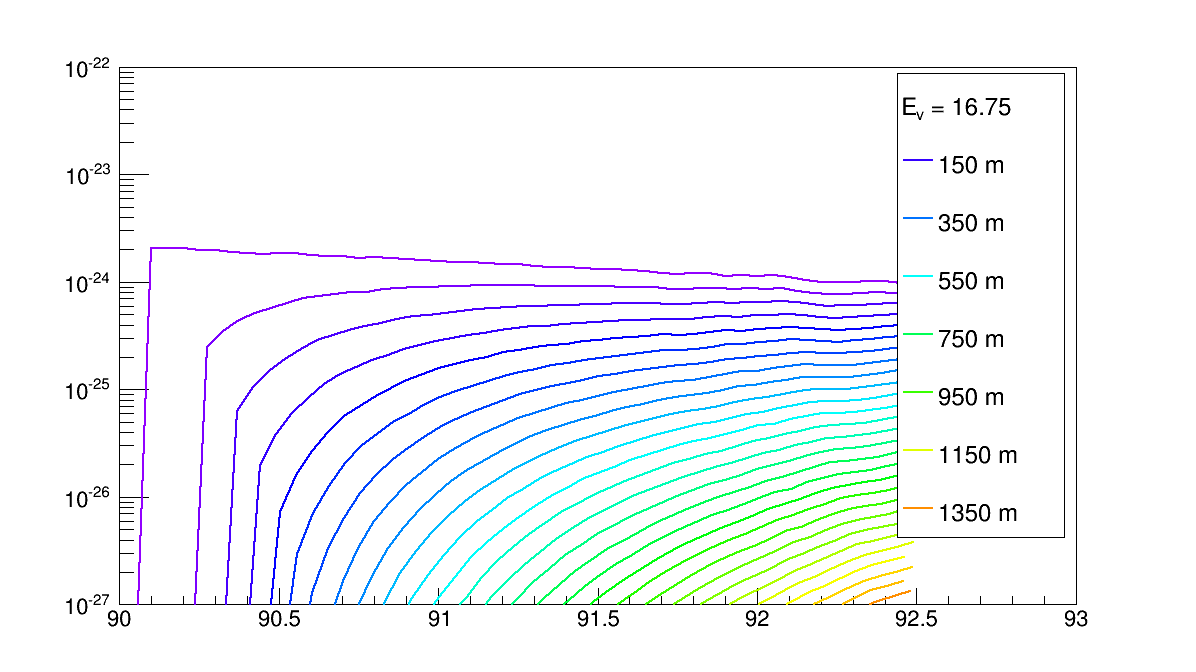
\includegraphics[width=0.45\textwidth]{fig/resultadosRadio/weights16_75.png} \\
		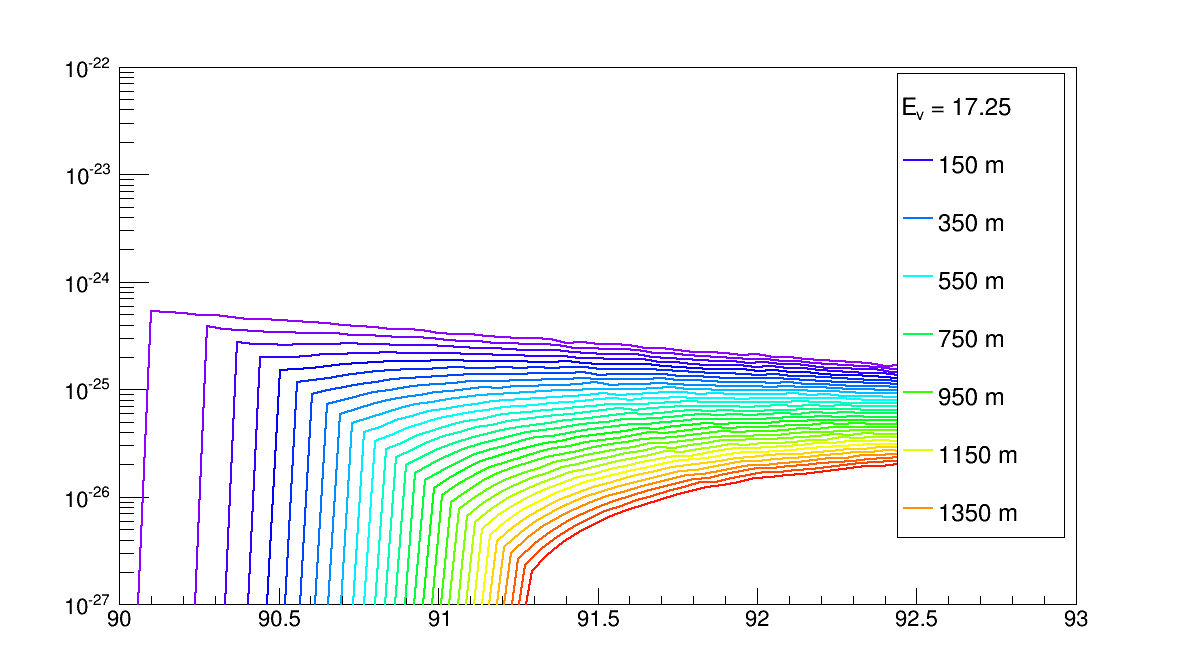
\includegraphics[width=0.45\textwidth]{fig/resultadosRadio/weights17_25.png} &
		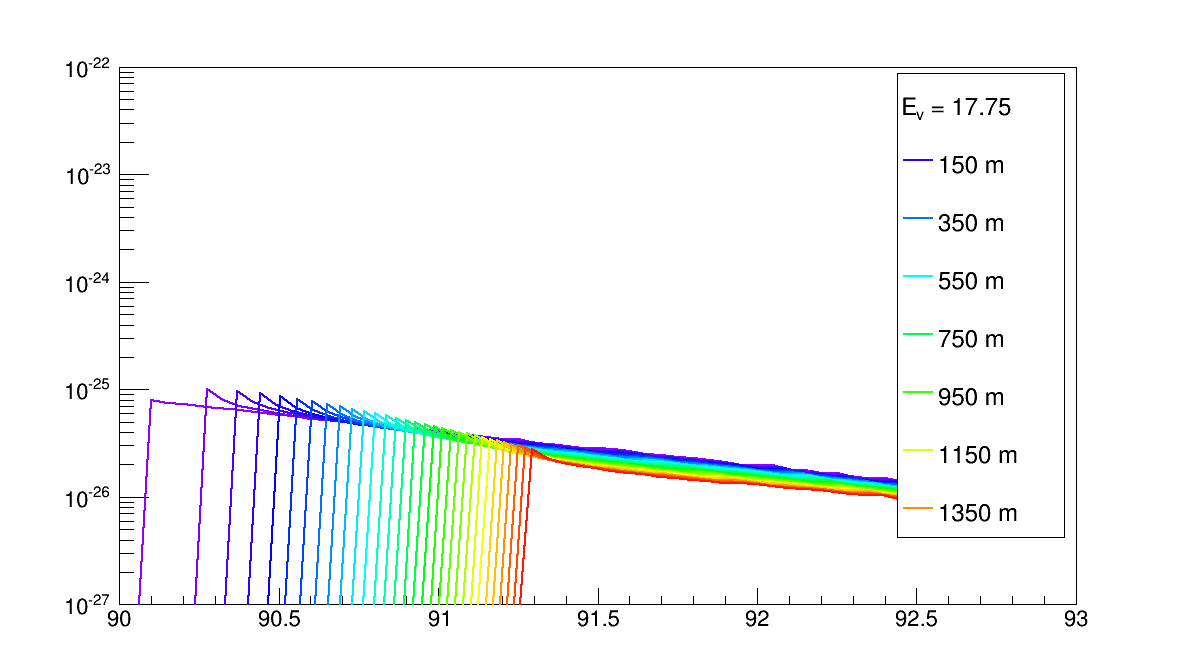
\includegraphics[width=0.45\textwidth]{fig/resultadosRadio/weights17_75.png} \\
		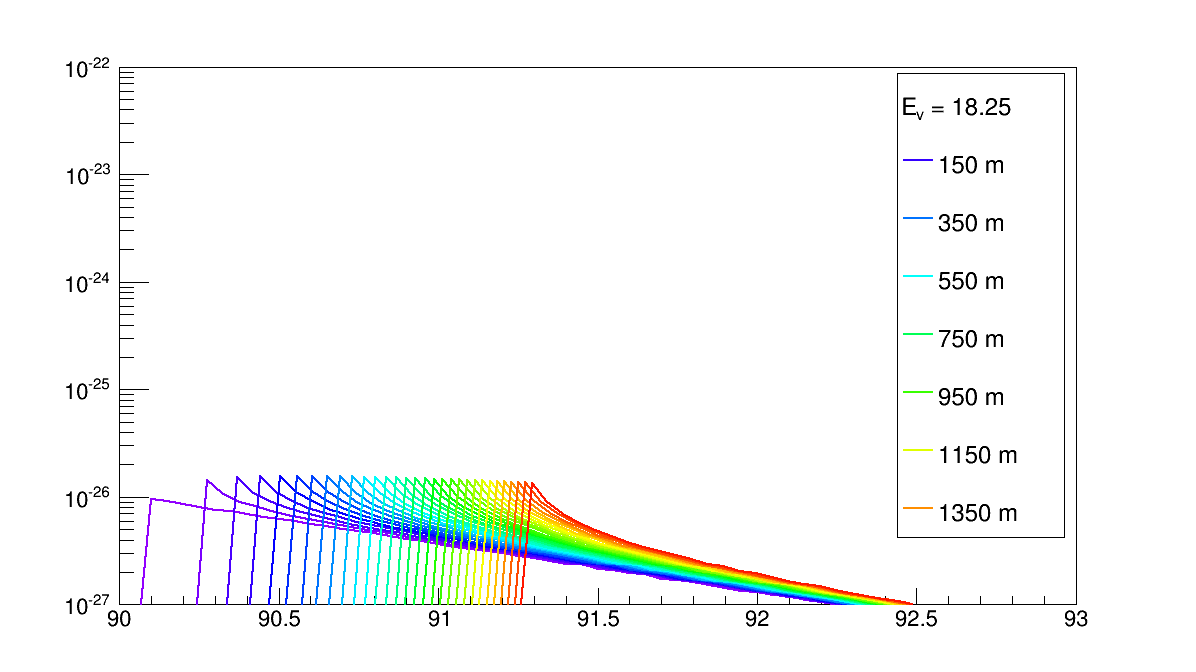
\includegraphics[width=0.45\textwidth]{fig/resultadosRadio/weights18_25.png} &
		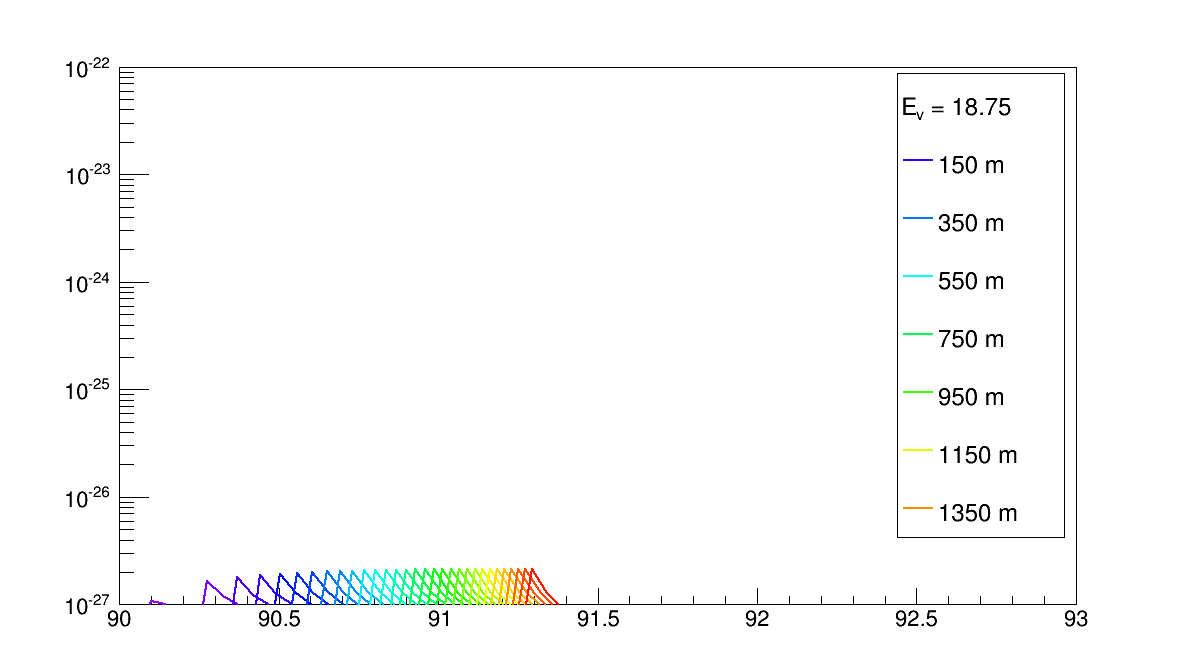
\includegraphics[width=0.45\textwidth]{fig/resultadosRadio/weights18_75.png} \\
		\end{tabular}

		\caption{\label{fig:radioShWeights}
		Probabilidad relativa  de las lluvias en funci\'on de la altura de decaimiento y el \'angulo cenital para diferentes valores de energ\'ia visible, suponiendo un flujo $\Phi(E_\nu)\propto E^{-2}$ y eficiencia m\'axima.
		Estos gr\'aficos muestran la importancia relativa en la exposici\'on de los diferentes bines de energ\'ia visibles, \'angulos cenitales y alturas de decaimiento.
		Por ejemplo, para $\sim90^\circ$ y \cant{150}{m} se esperan del orden de 100 veces m\'as eventos a \cant{10^{17.25}}{eV} que a \cant{10^{18.25}}{eV}.
		}
	\end{figure}
	
	Teniendo en cuenta todo lo anterior, y teniendo en cuenta el 
	\textbf{Justificar 1 lluvia por bin}
	La tabla \ref{tab:simRadio} muestra los bines simulados, es decir para  los cuales se calcular\'a la eficiencia de disparo.
	
	\subsubsection{Topograf\'ia del detector}
	
	Otro par\'ametro que afecta la eficiencia de disparo del detector es la disposici\'on espacial de las antenas, o topograf\'ia del detector.
	En este trabajo se consideraron varias opciones que ofrecen diversas ventajas y se enumeran a continuaci\'on.
	
	\begin{description}
	 \item[Regular:] asd
	 \item[Tipo pana\~n de abeja:] asd
	 \item[Bordes densos:] asd
	\end{description}
	
	
% 	\begin{figure}[h!]
% 		\begin{center}
% 		\begin{tabular}{cc}
% 			\cant{a_1=a_2=1000}{m}, $\alpha=90^\circ$ &
% 			\cant{a_1=a_2=1500}{m}, $\alpha=60^\circ$ \\
% 			\includegraphics[width=0.5\textwidth]{fig/resultadosRadio/{17.00_89.90_00.00_00025_01238_1000_1000_90_re}.pdf} &
% 			\includegraphics[width=0.5\textwidth]{fig/resultadosRadio/{17.00_89.90_00.00_00025_01238_1500_1500_60_re}.pdf} \\
% 			\cant{a_1=a_2=750}{m}, $\alpha=60^\circ$ &
% 			\cant{d=250}{m}, \cant{D=4000}{m} $\alpha=60^\circ$ \\
% 			\includegraphics[width=0.5\textwidth]{fig/resultadosRadio/{17.00_89.90_00.00_00025_01238_750_750_60_hc}.pdf} &
% 			\includegraphics[width=0.5\textwidth]{fig/resultadosRadio/{17.00_89.90_00.00_00025_01238_250_4000_90_de}.pdf}
% 		\end{tabular}
% 			\caption{asd}
% 			\label{fig:}
% 		\end{center}
% 	\end{figure}
	
	
	\subsubsection{M\'etodo de c\'alculo}
	
	\begin{figure}[ht!]
		\begin{center}
		\begin{tabular}{cc}
			\cant{a_1=a_2=1000}{m}, $\alpha=90^\circ$ \\
			\includegraphics[width=\textwidth]{fig/resultadosRadio/{17.00_89.90_00.00_00025_01238_1000_1000_90_re}.pdf} \\
			\cant{a_1=a_2=1500}{m}, $\alpha=60^\circ$ \\
			\includegraphics[width=\textwidth]{fig/resultadosRadio/{17.00_89.90_00.00_00025_01238_1500_1500_60_re}.pdf} \\
		\end{tabular}
			\caption{\label{fig:corePos1}
			Arriba, una grilla cuadrada de \cant{1000}{m} de paso. Abajo, una grilla hexagonal centrada de \cant{1500}{m} de paso como la del SD de Auger.
			En rojo se muestra la posici\'on del baricentro de la lluvia, lanzado al azar de 1000 dentro de la correspondiente celda primitva.
			}
		\end{center}
	\end{figure}
	
	\begin{figure}[ht!]
		\begin{center}
		\begin{tabular}{cc}
			\cant{a_1=a_2=750}{m}, $\alpha=60^\circ$ \\
			\includegraphics[width=\textwidth]{fig/resultadosRadio/{17.00_89.90_00.00_00025_01238_750_750_60_hc}.pdf} \\
			\cant{d=500}{m}, \cant{D=4000}{m} $\alpha=60^\circ$ \\
			\includegraphics[width=\textwidth]{fig/resultadosRadio/{17.00_89.90_00.00_00025_01238_500_4000_90_de}.pdf}
		\end{tabular}
			\caption{\label{fig:corePos2}
			Arriba, una grilla hexagonal tipo panal de abeja de \cant{750}{m} de paso. Abajo, una de tipo bordes densos de \cant{4000}{m} de paso y \cant{500}{m} de paso interno.
			Nuevamente en rojo se muestra la posici\'on del baricentro de la lluvia, lanzado al azar de 1000 dentro de la correspondiente celda primitva.}
		\end{center}
	\end{figure}
	
	\begin{figure}[h!]
		\begin{center}
			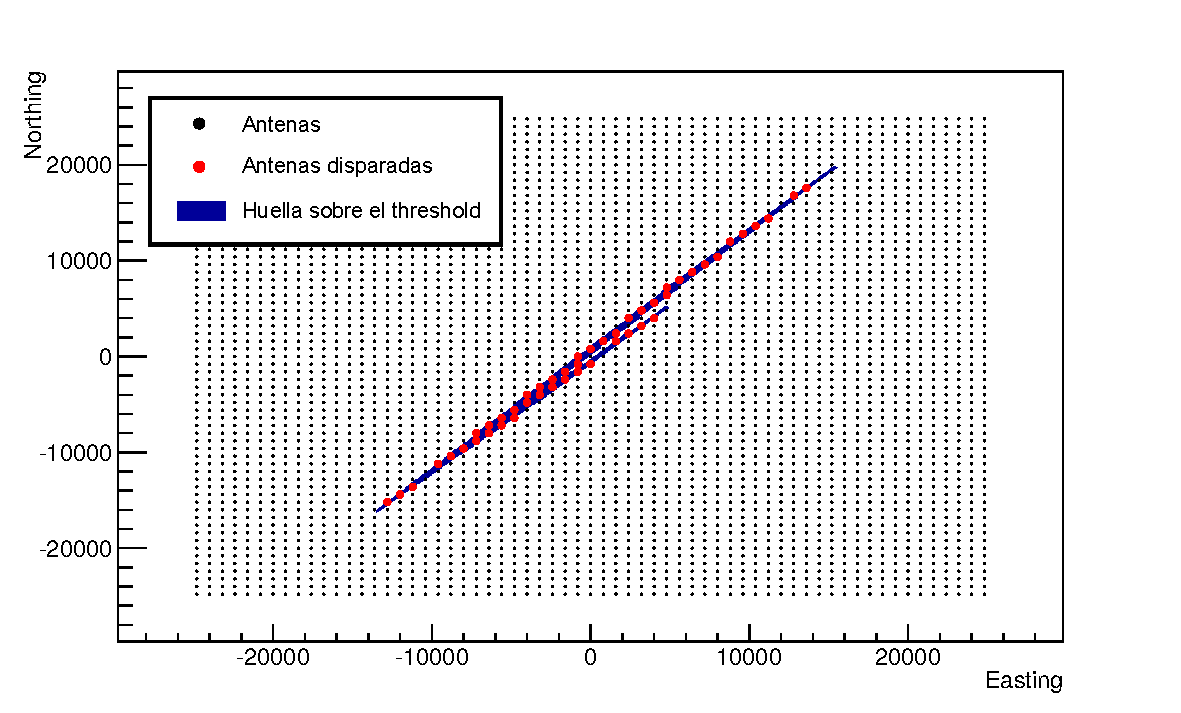
\includegraphics[width=\textwidth]{fig/resultadosRadio/trigger}
			\caption{asd}
			\label{fig:}
		\end{center}
	\end{figure}
	
	definicion del threshold
	
	descarte del canal muonico
	
% 	reescaleo por identificacion
	
	\begin{figure}[h!]
		\begin{center}
				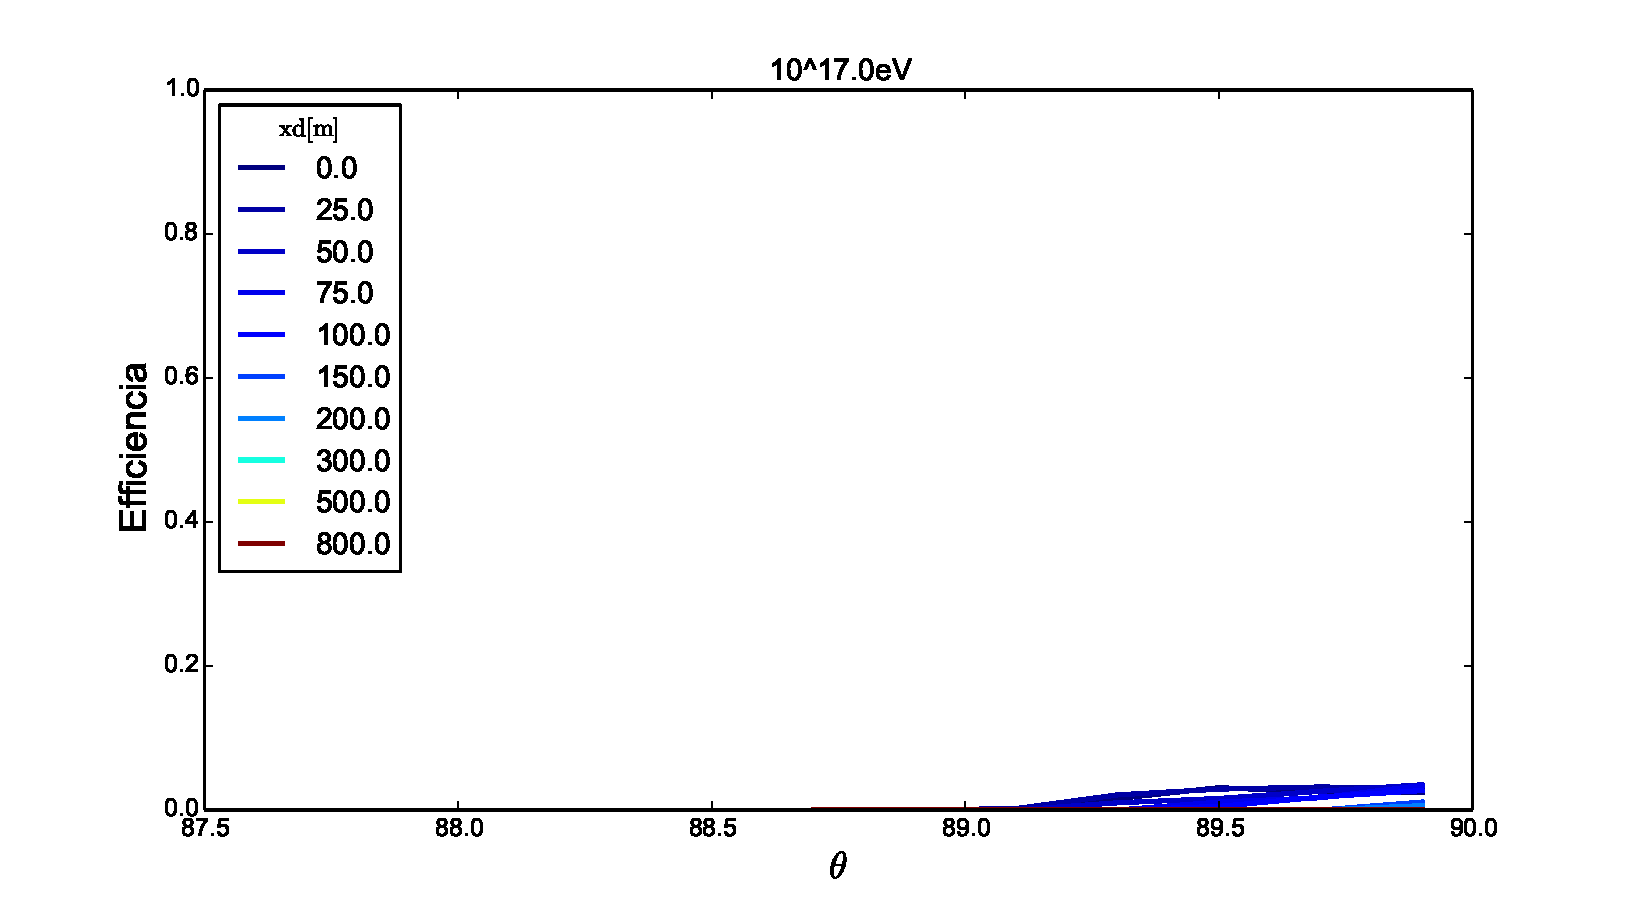
\includegraphics[width=0.9\textwidth]{fig/resultadosRadio/eff75_0_4_0_1500_0_1500_0_60_0_1_0_17_0_m2.pdf} 
				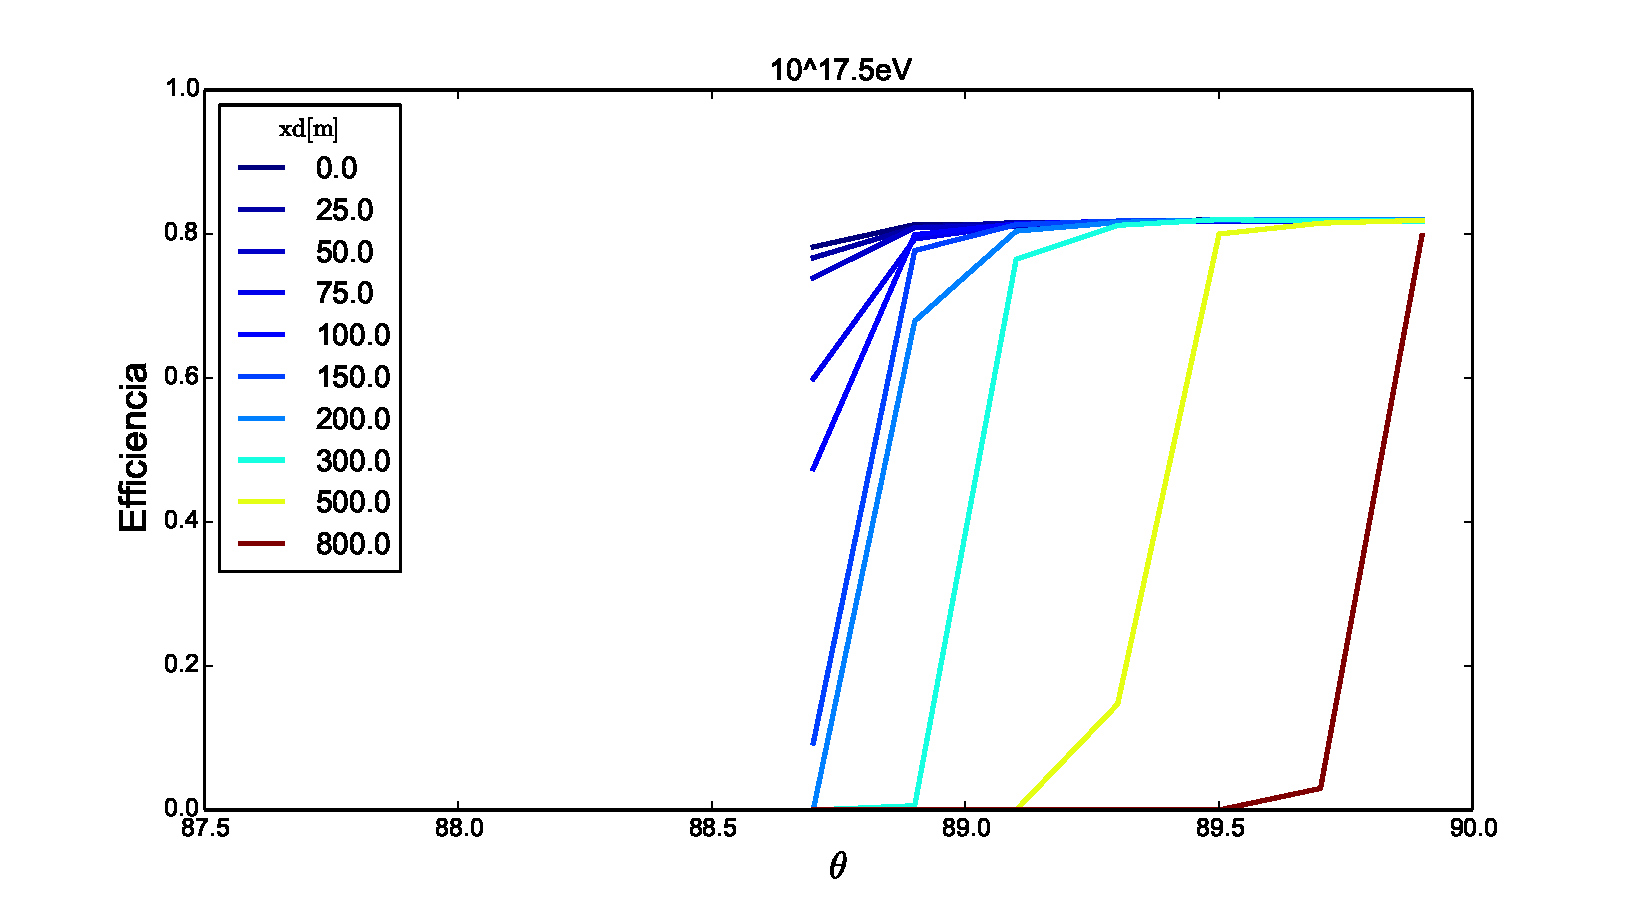
\includegraphics[width=0.9\textwidth]{fig/resultadosRadio/eff75_0_4_0_1500_0_1500_0_60_0_1_0_17_5_m2.pdf}
				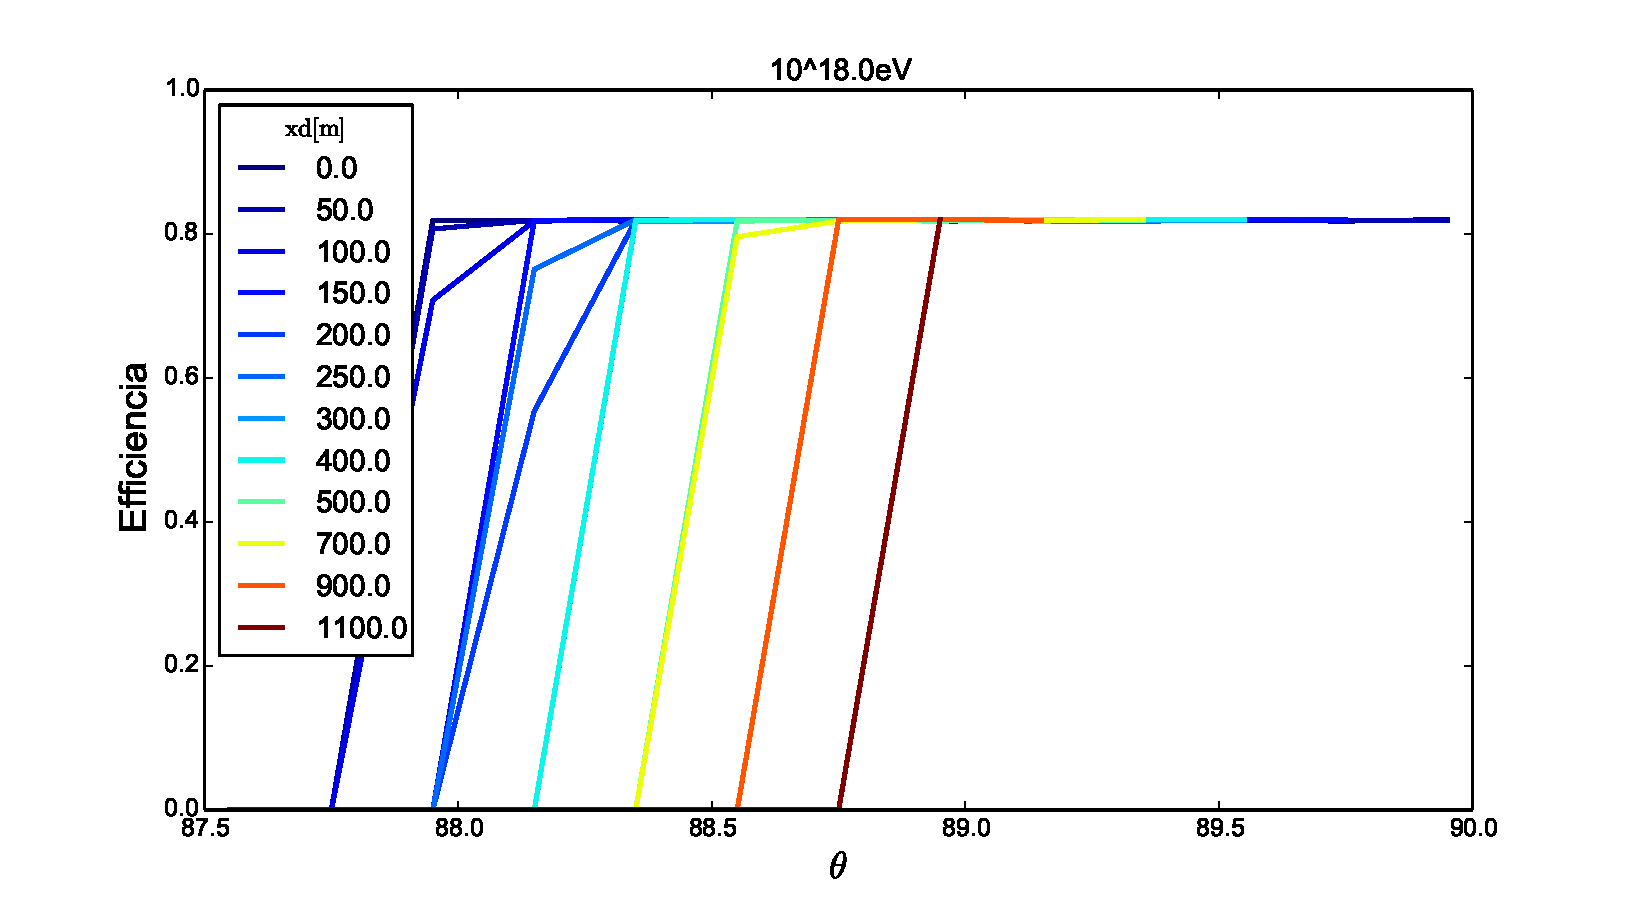
\includegraphics[width=0.9\textwidth]{fig/resultadosRadio/eff75_0_4_0_1500_0_1500_0_60_0_1_0_18_0_m2.pdf}
			\caption{asd}
			\label{fig:}
		\end{center}
	\end{figure}
	
	\begin{figure}[h!]
		\begin{center}
% 		\begin{ta
			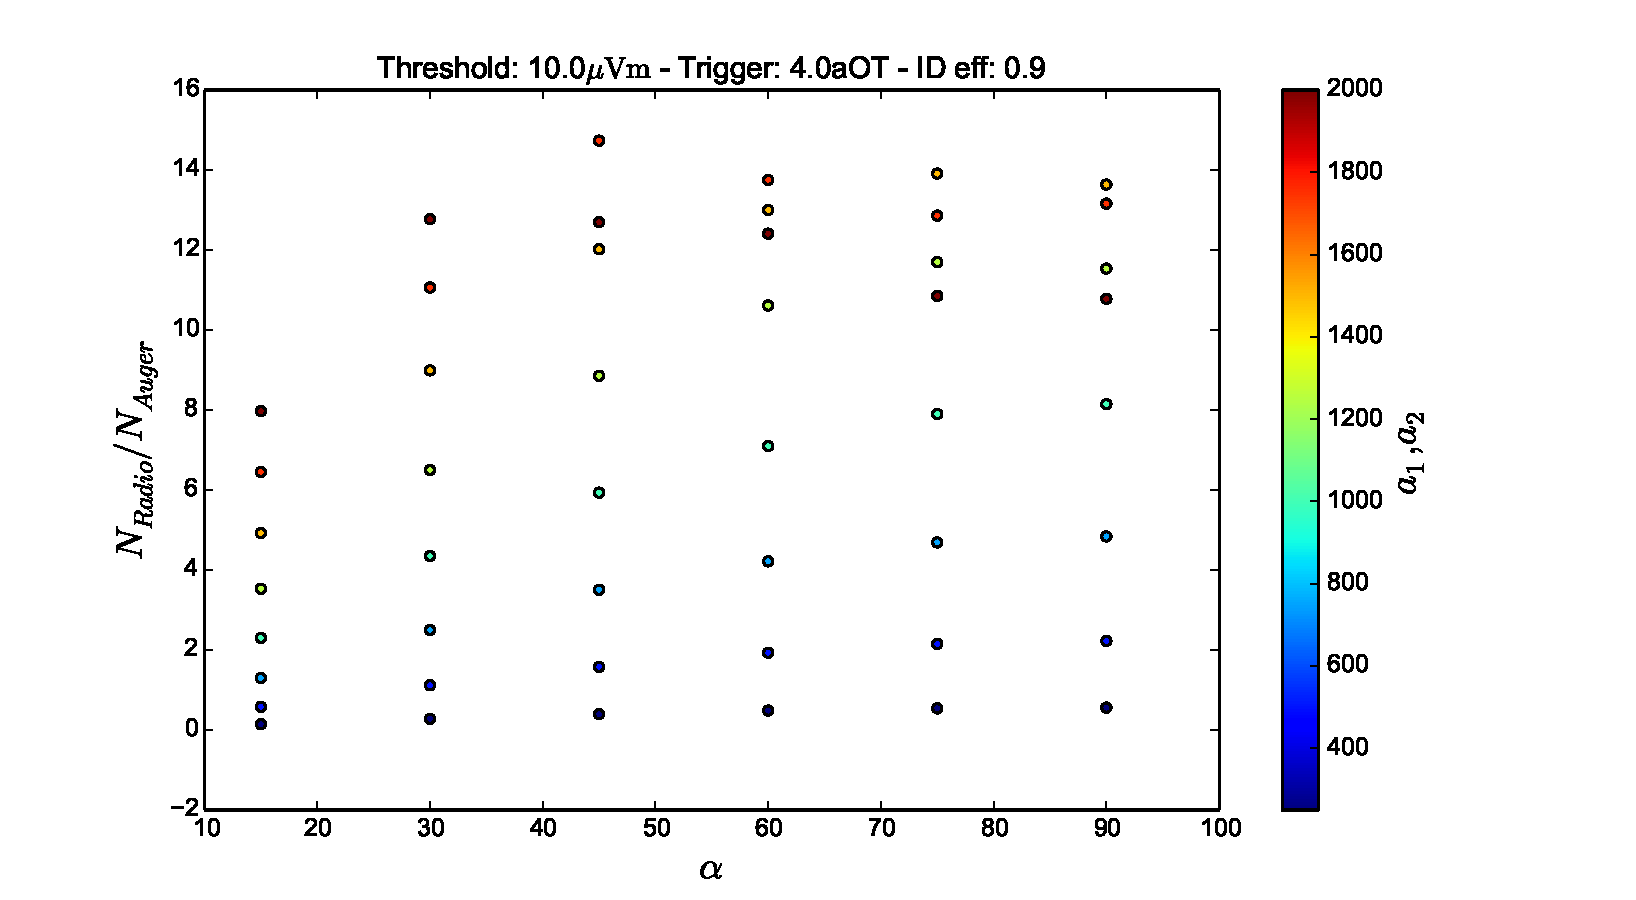
\includegraphics[width=0.7\textwidth]{fig/resultadosRadio/CompRadioAuger_10_0_4_0_0_9_hc_modo1.pdf}
			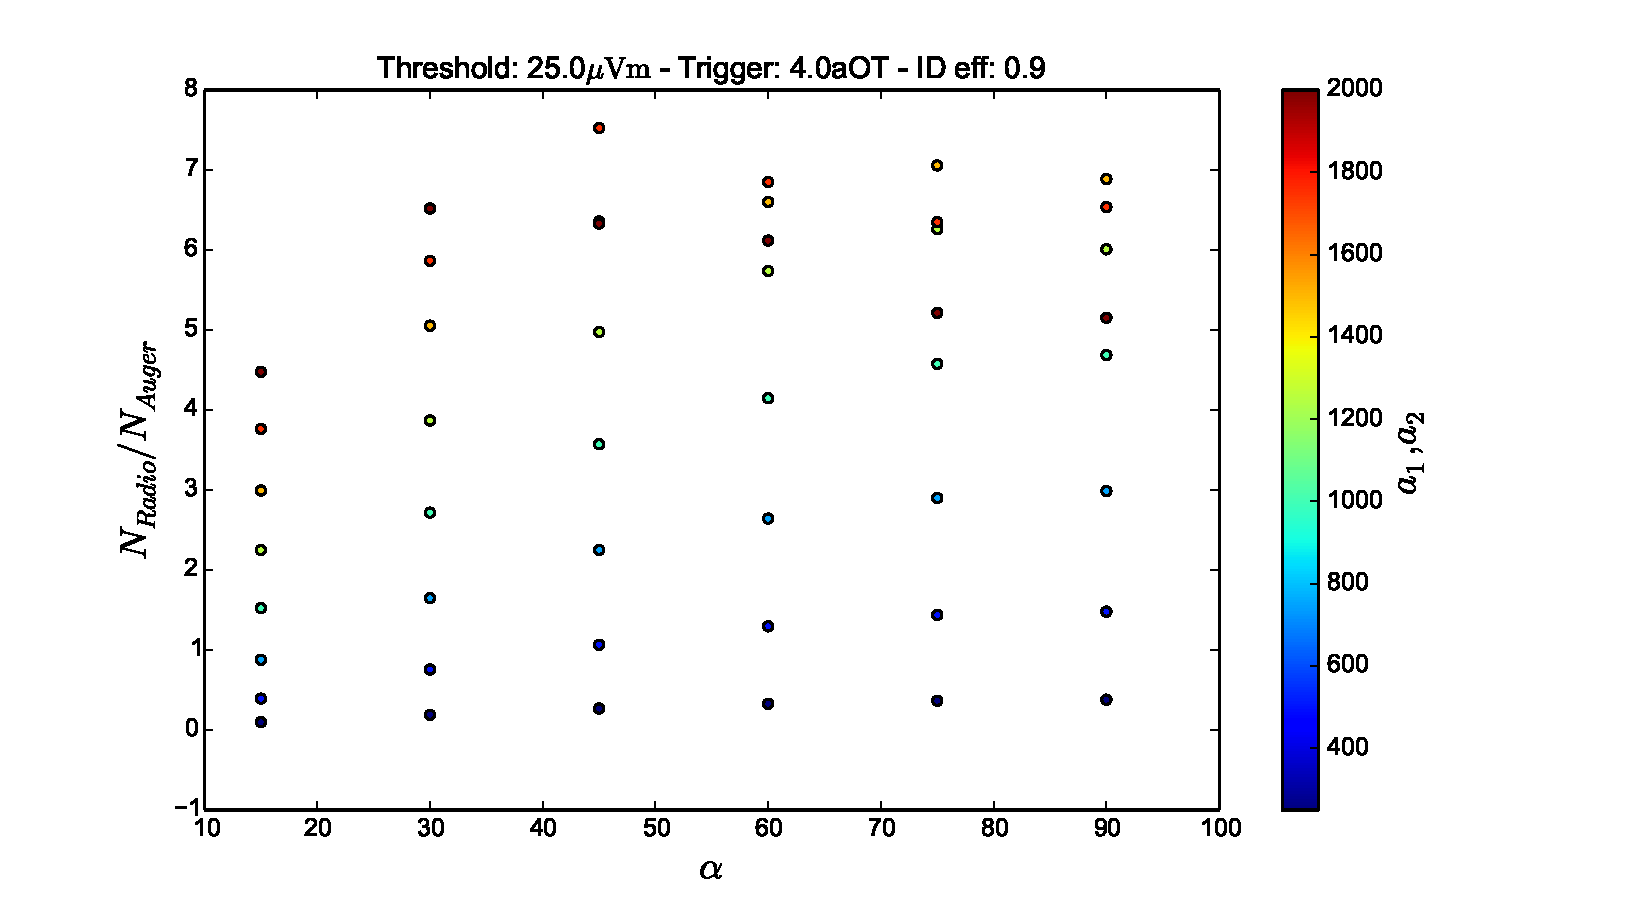
\includegraphics[width=0.7\textwidth]{fig/resultadosRadio/CompRadioAuger_25_0_4_0_0_9_hc_modo1.pdf}
			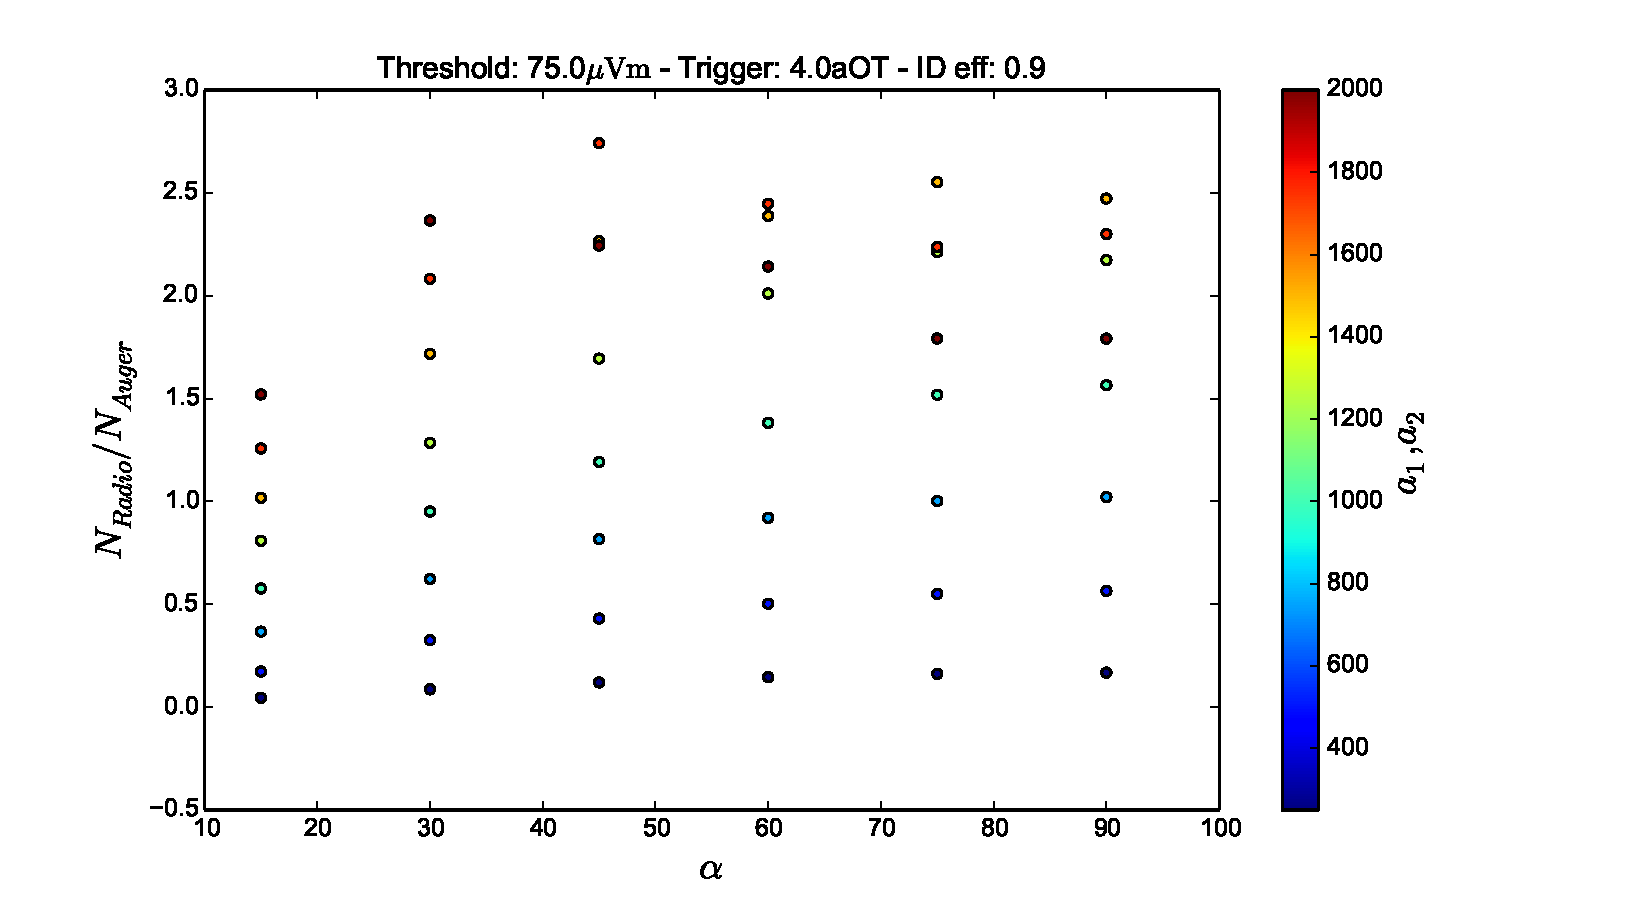
\includegraphics[width=0.7\textwidth]{fig/resultadosRadio/CompRadioAuger_75_0_4_0_0_9_hc_modo1.pdf}
			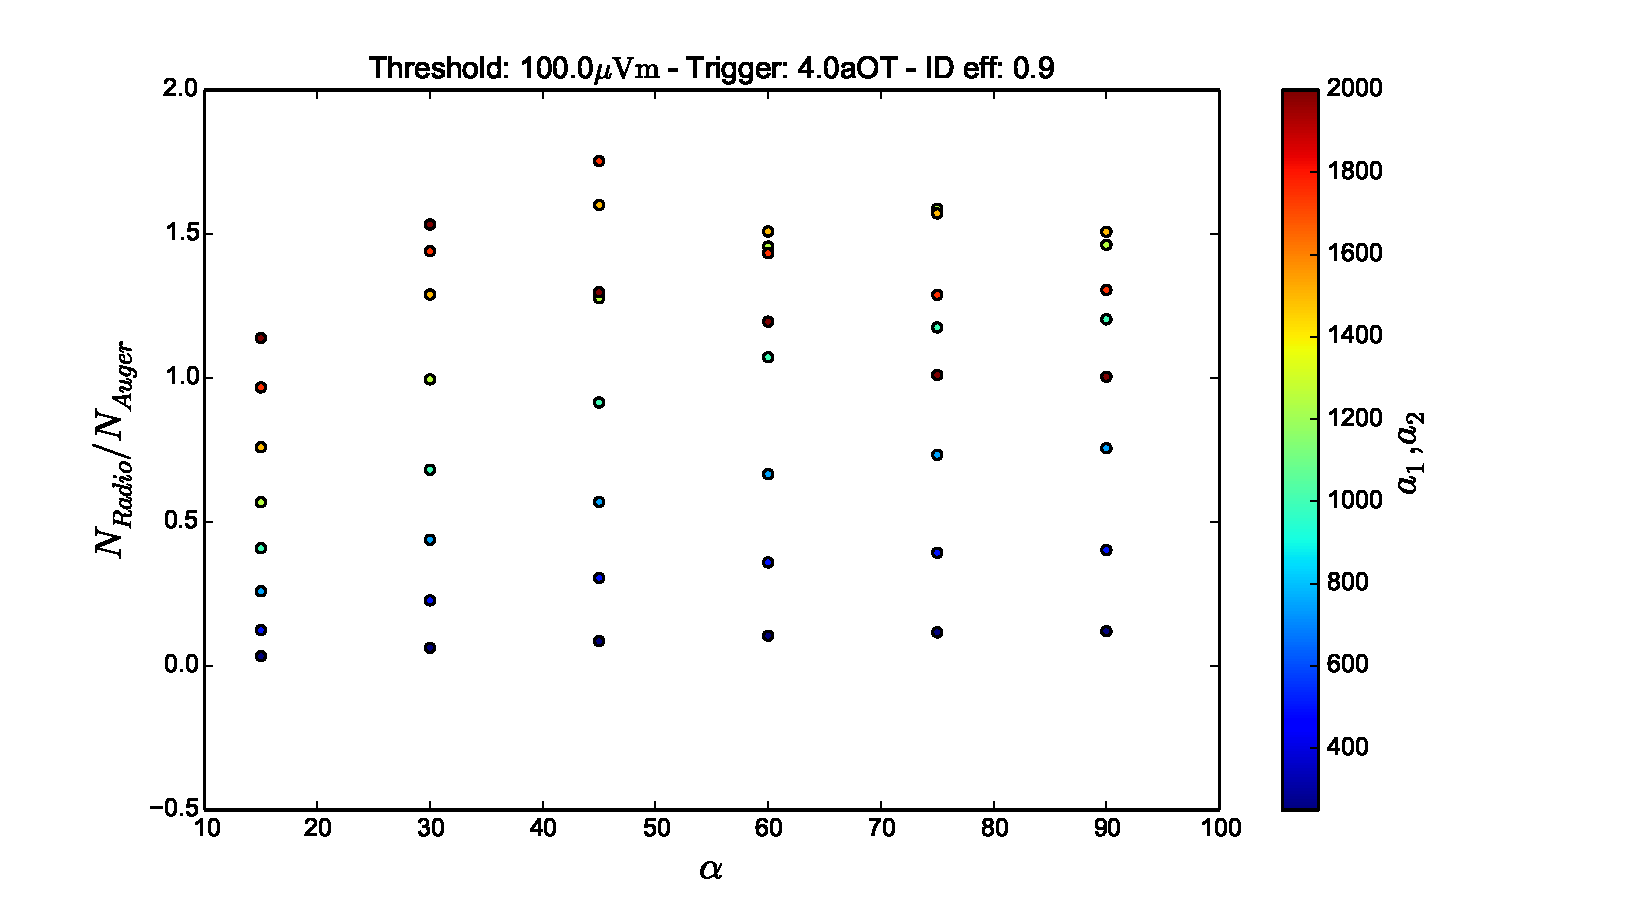
\includegraphics[width=0.7\textwidth]{fig/resultadosRadio/CompRadioAuger_100_0_4_0_0_9_hc_modo1.pdf}
			\caption{asd}
			\label{fig:}
		\end{center}
	\end{figure}
	
	
	\subsection{Eficiencias de identificaci\'on - Discriminaci\'on en el fondo de eventos hadr\'onicos}
	\label{sc:identificacionRadio}

	Como se expuso en la primer parte de esta tesis, el mayor desaf\'io a la hora de detectar neutrinos ES mediante detectores de superficie resulta ser su discriminaci\'on en el fondo dominante de eventos hadr\'onicos.
	En Auger esto se logra debido a que los tanques \cher{} permiten detectar las lluvias j\'ovenes entre los eventos inclinados, a trav\'es de variables sensibles a la presencia de componente electromagn\'etica.
	En un detector de antenas de radio esta separaci\'on no resulta posible debido a que b\'asicamente toda la emisi\'on es generada en el m\'aximo de la lluvia por los electrones de media y baja energ\'ia.
	Sin embargo, su geometr\'ia permite salvar este escollo, ya que guarda informaci\'on sobre la ubicaci\'on en la que se produjo dicho m\'aximo.
	Para clarificar la situci\'on, en la figura \ref{fig:dg_vs_es_radio} se representa la emisi\'on \cher{} de un evento DG inclinado (un evento de background), y uno ES.
	%
	\begin{figure}[ht!]
		\centering
		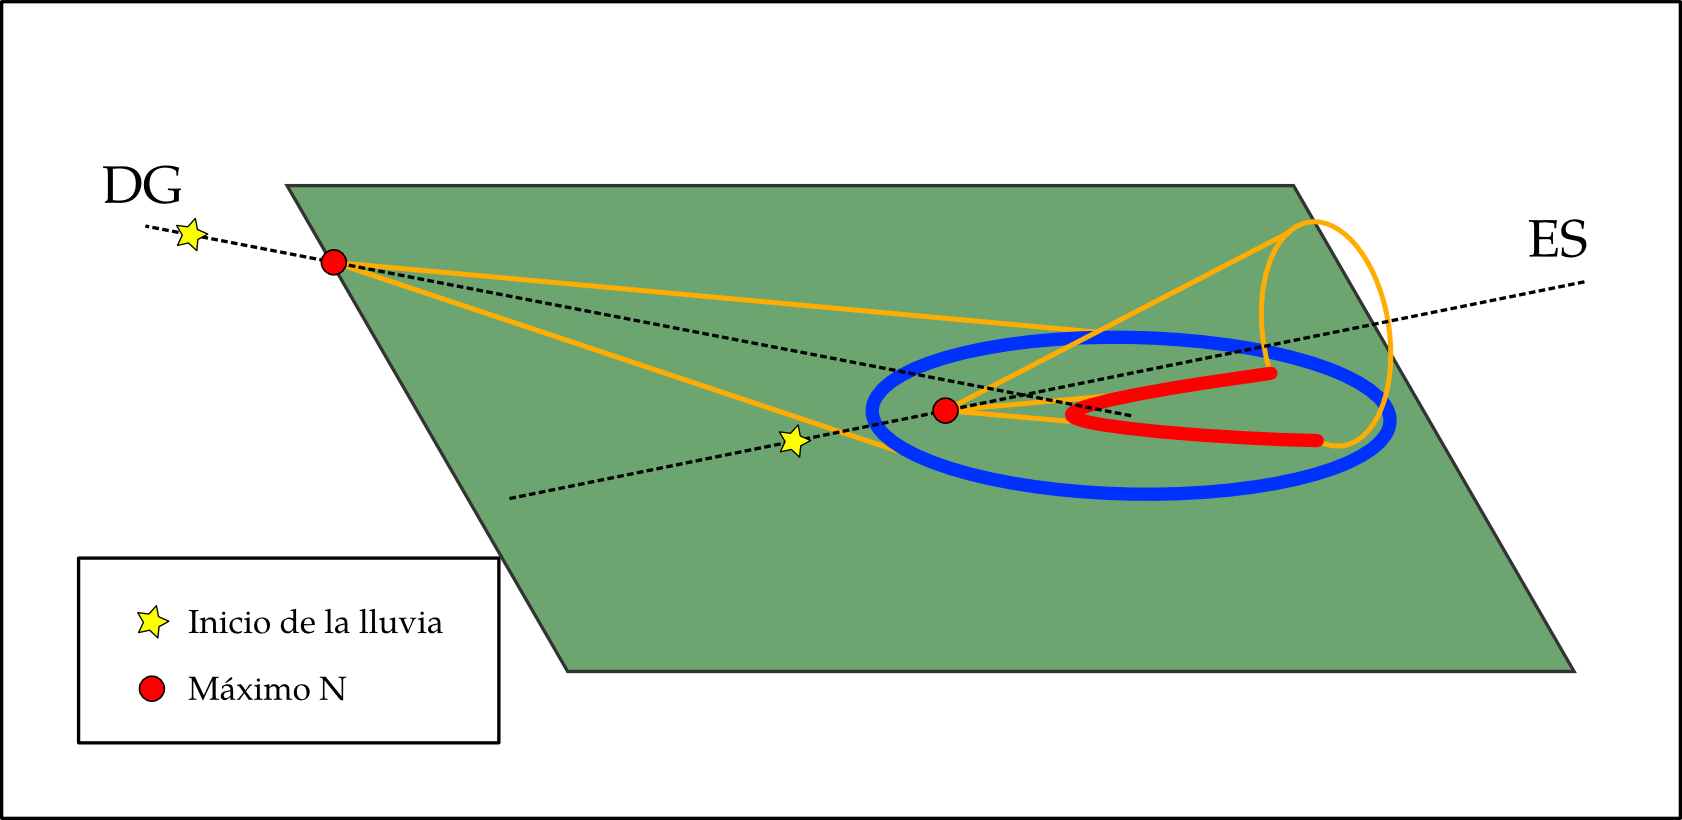
\includegraphics[width=\textwidth]{./fig/simulacionRadio/idRadio.png}
		\caption{\label{fig:dg_vs_es_radio}
		Esquema de las caracter\'isticas que permiten distinguir los eventos ES del fondo de lluvias hadr\'onicas horizontales (DG). Dado que las lluvias DG se inician alto en la atm\'osfera la apertura del cono \cher{} al nivel de la superficie (l\'inea azul) resulta mucho mayor que la que alcanzar\'ia en un evento ES, debido a que su m\'aximo se produce mucho m\'as cerca de la superficie.
	% 	Adem\'as de la apertura del cono, otro posible factor de discriminaci\'on puede ser la topograf\'ia de la se\~nal a nivel del suelo, ya que en los eventos DG imprimen elipses y los ES hip\'erbolas.
		}
	\end{figure}
	%
	La apertura del cono del evento DG a nivel del suelo resulta mayor que la que imprime el evento ES.
	Esto se debe a que los eventos hadr\'onicos inclinados se inician cerca del tope de la atm\'osfera, por lo que la emisi\'on debe recorrer hasta 36 atm\'osferas antes de alcanzar el detector.
	De esta manera, el cono \cher{} es cortado por el detector mucho m\'as lejos de su v\'ertice (que resulta ser aproximadamente el m\'aximo de la lluvia) que en eventos ES, los que se desarollan mucho m\'as cerca del detector.

	Para dar sustento a esta conjetura fue necesario simular eventos hadr\'onicos descendentes.
	Debido a 
	que se muestran en la figura \ref{fig:dg_thetas}.

		\begin{figure}[ht!]
			\centering
			\begin{tabular}{cc}
			$\theta_D=85^\circ$ & $\theta_D=87^\circ$ \\
			\includegraphics[width=0.5\textwidth]{./fig/resultadosRadio/dg/{foorPrint_ZWv1.33_ntuples_v1.22_Downgoing_phi_90_19.5_85_90_100_1_E}.png} &
			\includegraphics[width=0.5\textwidth]{./fig/resultadosRadio/dg/{foorPrint_ZWv1.33_ntuples_v1.22_Downgoing_phi_90_18.5_87_90_100_2_E}.png}\\
			
			$\theta_D=88^\circ$ & $\theta_D=89^\circ$ \\
			\includegraphics[width=0.5\textwidth]{./fig/resultadosRadio/dg/{foorPrint_ZWv1.33_ntuples_v1.22_Downgoing_phi_90_18.5_88_90_100_6_E}.png} &
			\includegraphics[width=0.5\textwidth]{./fig/resultadosRadio/dg/{foorPrint_ZWv1.34_ntuples_v1.22_Downgoing_phi_90_18.5_89_90_100_5_E}.png}\\
			\end{tabular}
			\caption{\label{fig:dg_thetas}
			Huella sobre el detector
			}
		\end{figure}

	6800 horas cpu
	% 
	% 
	% Tambi\'en, se nota como la opograf\'ia de la huella en ambos casos es fundamentalmente distinta, ya que el evento DG imprime una elipse sobre el suelo y el evento ES una hip\'erbola.
	% En consecuencia se estudiar\'a si es posible explotar estas diferencias para identificar eventos ES.

	Por otra parte, en la figura 

	- eventos gigantes

	- se inician lejos y el campo cae como 1/R pero el drift es mayor debido a la baja densidad de la atm\'osfera

	- ver v4.20 en ntuple analizer mostrar que la velocidad sobre el eje y el ancho 

\subsubsection{Resumen del an\'alisis de la se\~nal}

	\begin{table}[ht!]
	\centering
	\begin{tabular}{|p{0.3\textwidth}|p{0.7\textwidth}|}
	\toprule
	Descripci\'on & Detalle \\
	\midrule\midrule
	Filtrado de la se\~nal & Respuesta plana en la banda \cant{30\text{-}80\text{/}120\text{-}900}{MHz} \\ \midrule
	Nivel de disparo local &  Entre \cant{25}{\frac{\mu V}{m}} y \cant{200}{\frac{\mu V}{m}} con un paso de \cant{25}{\frac{\mu V}{m}}\\ \midrule
	Disparo global & Antenas disparadas compatibles con un frente que se desplaza a la velocidad de la luz \\ \midrule
 	Nivel de identificaci\'on & Eficiencia entre 0.80 y 1.00 con un paso de 0.05 \\
	
	\bottomrule
	\end{tabular}
	\end{table}

	
\section{Desempe\~no de un detector de 90000 antenas}

El objetivo de esta secci\'on es discutir la posibilidad de armar un detector de 10000 antenas de radio cuyo fin ser\'ia detectar neutrinos ES.
Para ello, ser\'a necesario utilizar toda la informaci\'on racavada hasta el momento, as\'i como analizar las diferentes topolog\'ias con las que se podrian distribuir 


	\begin{figure}[h!]
		\begin{center}
			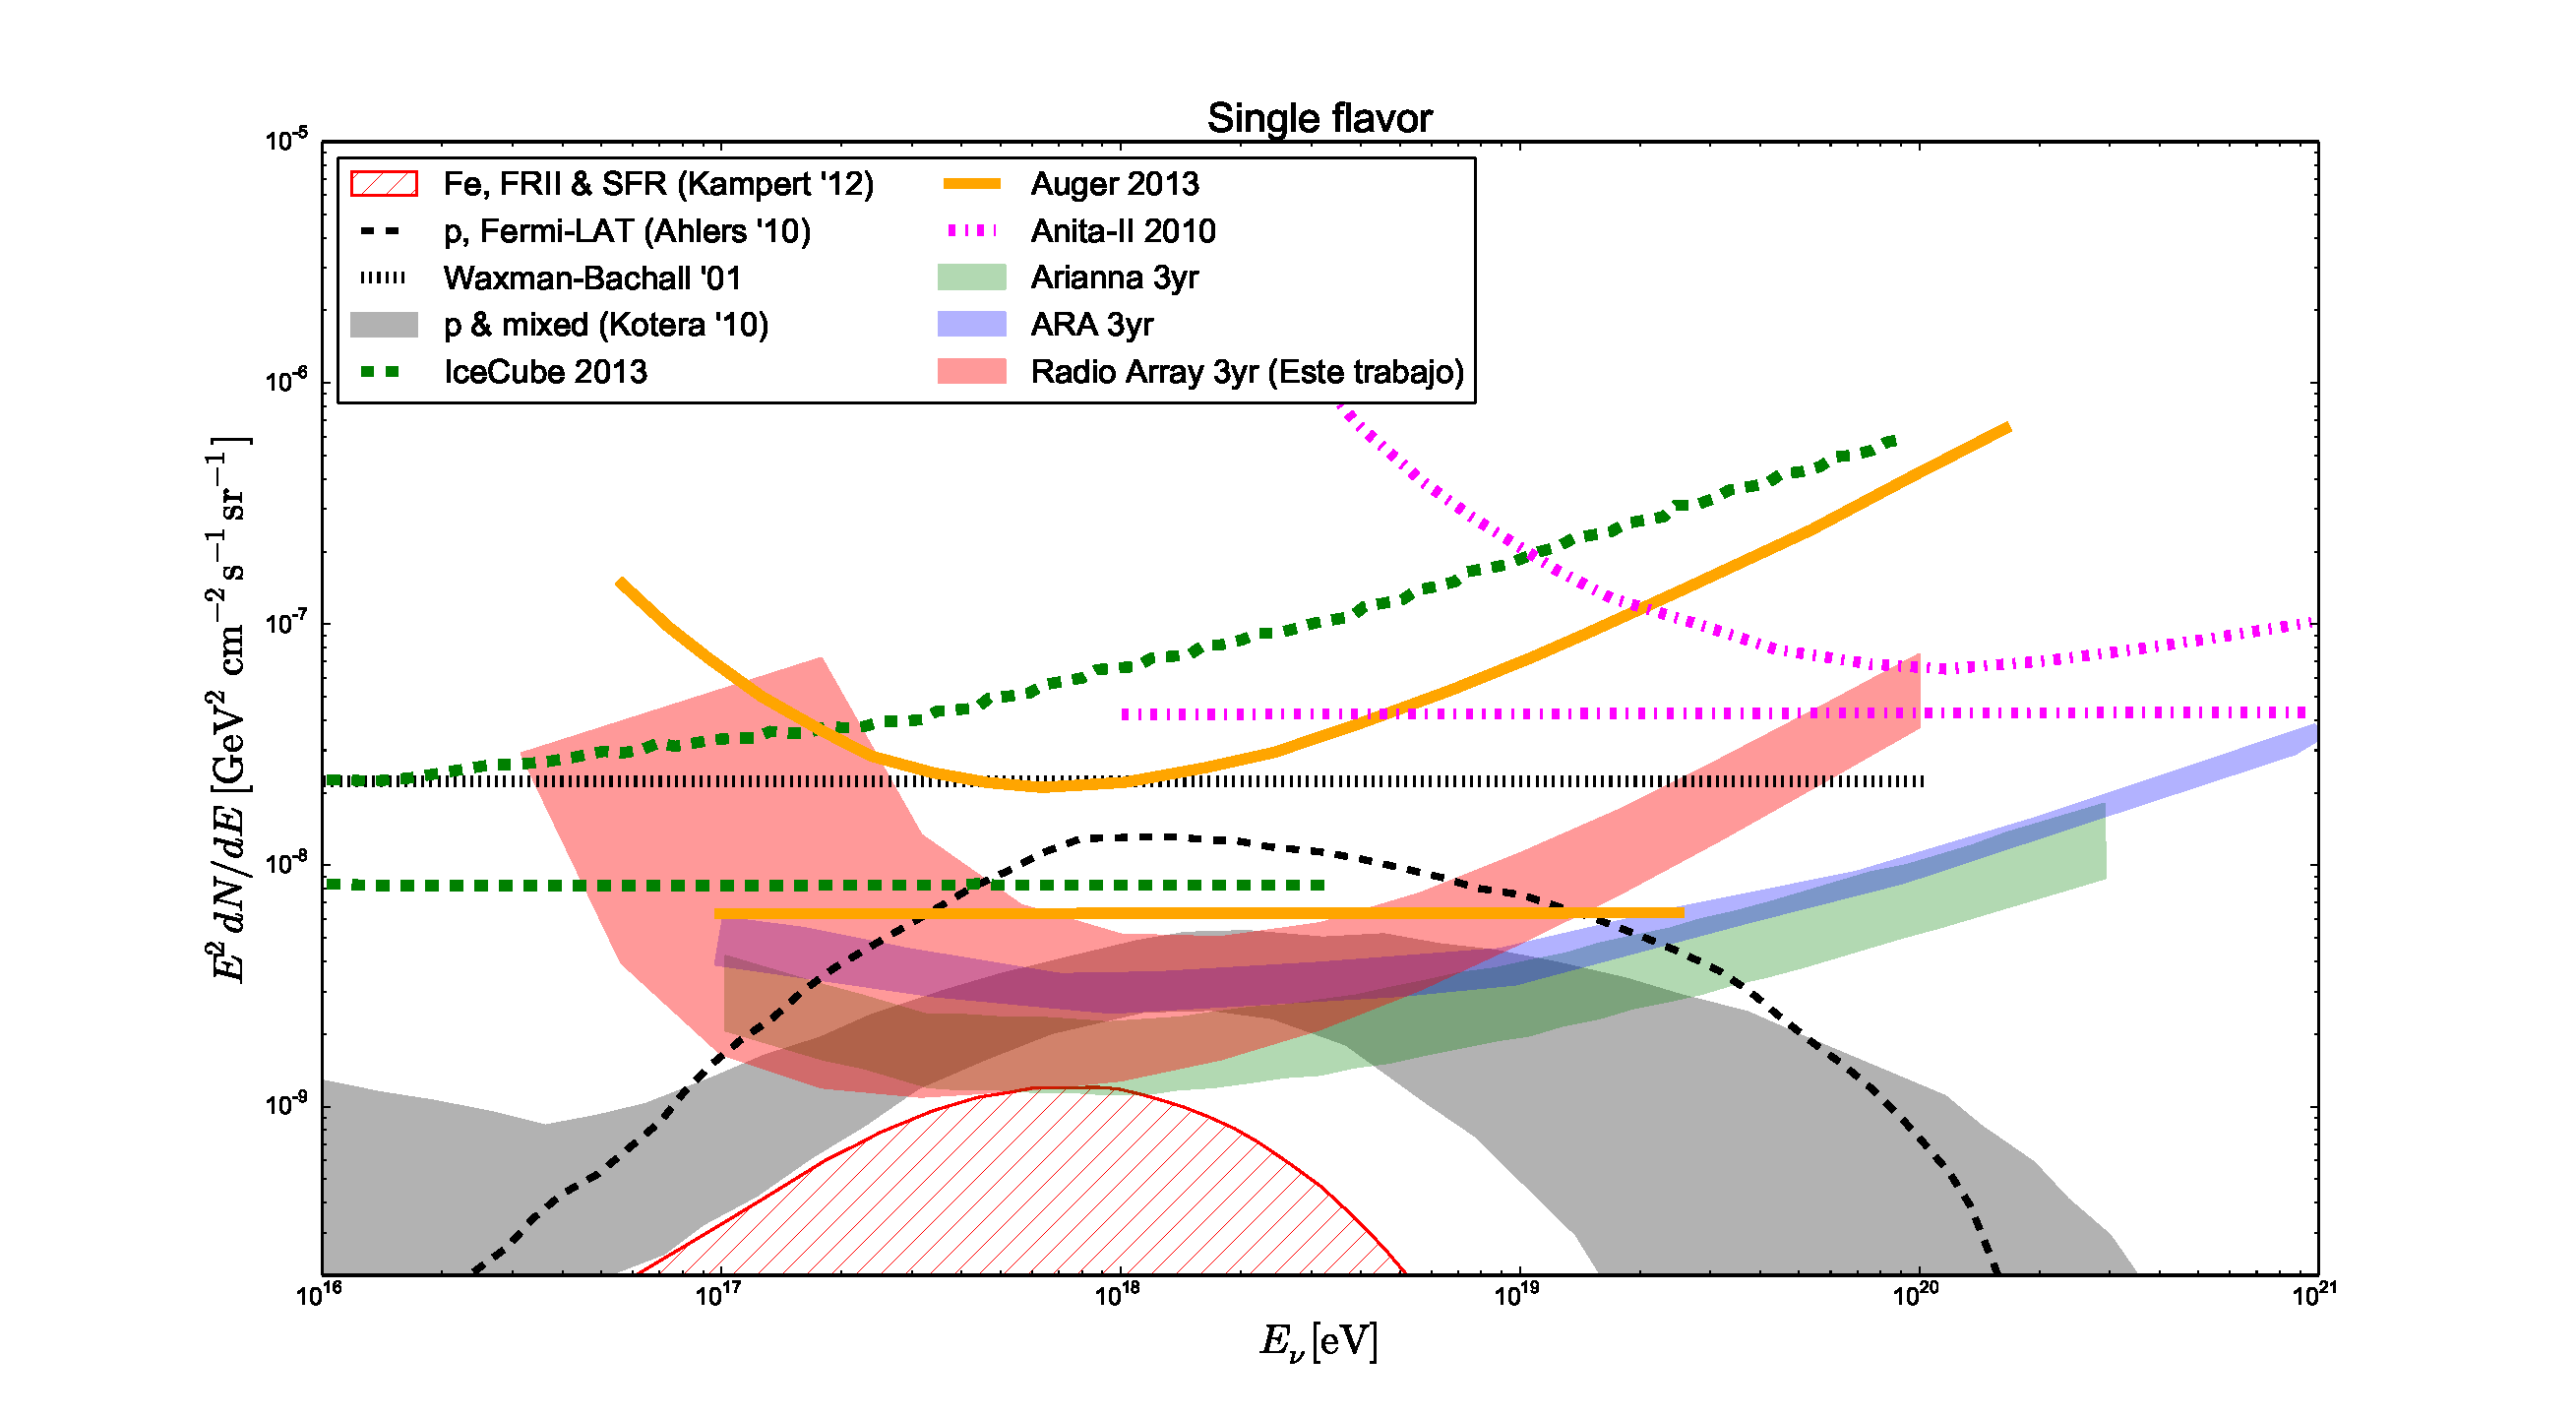
\includegraphics[width=\textwidth]{fig/resultadosRadio/limits_future}
			\caption{asd}
			\label{fig:}
		\end{center}
	\end{figure}